\appendix
\section*{Appendix}
The organization of the appendix are as follows.
In \appxref{related}, we briefly discuss the related work relevant to our research.
In \appxref{background}, we review some background knowledge of Riemannian geometry and stochastic calculus on the manifold. In \appxref{rigorous-construction}, we give the details of the Riemannian structures of the quotient space. In \appxref{proofs}, we give all the proofs of the theorems in the main text. In \appxref{general-method}, we show our methods for the general case. In \appxref{add-exp}, we give some additional results and discussions. Finally, the details of the experiments are given in \appxref{experiments}.

\section{Related Work}
\label{appx:related}
\paragraph{Diffusion models on Riemannian manifolds.} As the quotient has the Riemannian manifold structure, several previous works construct the diffusion model on the Riemannian manifolds. \citet{de2022riemannian} constructs diffusion models using different overlapping local coordinate systems of the manifold and requires geodesic random walk to simulate the forward process. \citet{huang2022riemannian,chen2023flow} construct diffusion models in an embedding space which allows a global representation but requires explicit geodesic formula of the manifold. %\textcolor{blue}{
\citet{zhu2024trivialized} constructs the reverse of kinetic Langevin dynamics on a Lie group to perform generative modeling. % In their framework, the Brownian motion term is added only on the tangent space of the Lie group, which is trivialized as an Euclidean space.}
Such an approach is not designed for and not readily applicable to the quotient space, which has a different geometric structure from the Lie group.
In our quotient space case, the specialty with a quotient structure enables us to construct diffusion models using the coordinate systems of the total space without relying on an embedding of the quotient in the total space (unnecessarily an embedding space), which is more practical to implement yet still general.

\paragraph{Geometric diffusion models.} 
To ensure physical symmetry in the generation process, a mainstream strategy integrates fundamental physical constraints, such as SE(3) equivariance, directly into the diffusion-model architecture. This approach, pioneered by models like EDM~\citep{hoogeboom2022equivariant}, typically employs an EGNN to operate directly on atomic coordinates, using techniques like zero center of mass adjustments to guarantee translational invariance. This foundational concept was subsequently extended in several directions. For instance, the approach was adapted for Diffusion Bridges in models like EDM-Bridge~\citep{wu2022diffusion} and for diffusion in a latent space in models like GeoLDM~\citep{xu2023geometric}. These equivariant diffusion techniques have been successfully applied across a range of molecular tasks. For structure generation, models like GeoDiff~\citep{xu2022geodiff} predict 3D structures from molecular graphs. In molecular optimization, methods such as DiffHopp~\citep{torge2023diffhopp} refine existing molecules to enhance desired properties. For de novo design, a key advancement has been to combine discrete diffusion models (D3PM)~\citep{austin2021structured} for 2D topology with continuous equivariant diffusion for 3D geometry, enabling joint generation as seen in models like DiffSBDD~\citep{schneuing2024structure} and MUDiff~\citep{hua2024mudiff}. % \textcolor{blue}{
A similar problem has also been considered in crystalline structure generation, where the intrinsic periodic translation invariance is an intrinsic symmetry. \citet{lin2024equivariant} highlighted the intrinsic periodic translation symmetry that has been omitted for a long time in the field of periodic crystalline structure generation. The work designed a modified diffusion process that induces a transition kernel that is invariant under periodic translation, %. The resulting optimization problem, while keeping the simplicity of no data augmentation,
leading to a learning target for the score model that is invariant under periodic translation. \citet{cornet2025kinetic} proposes a novel method that generalizes the Trivialized Diffusion Model framework for fractional coordinates to model the intrinsic periodic translation symmetry using flat coordinates. The proposed method considers the process with the velocity restricted to the CoM-free linear subspace. % Although considering different generation tasks, both works have a similar motivation to reduce the learning difficulty of the model using the intrinsic symmetry of the data distribution. %}
They have achieved the removal of variance on equivalent DoFs, but still asks the neural network model to learn to predict a specific target in the equivalent DoFs.

\paragraph{Learning with alignment}
To reduce learning difficulty, some heuristic treatments (learning with alignment) have been proposed in hope to reduce the DoFs corresponding to the symmetry group action. The alignment strategy used in GeoDiff~\citep{xu2022geodiff} aligns the target structure to the noisy input by finding an optimal rigid transformation that minimizes the distance between them. Another approach, proposed in AlphaFold~3 (AF3)~\citep{abramson2024accurate}, aligns the target samples to the model output structure. As discussed in the main text, these two alignment-based training frameworks lack a definite guarantee for recovering the correct target distribution, and is incompatible with the sampling process. Boltz-1~\citep{wohlwend2025boltz}, an open-source replication of AF3, noticed this issue and proposed a modification in sampling to align the denoised structure to the structure in the current generation step before updating. Nevertheless, as discussed in \secref{comparison}, this, together with the training protocol of AF3, amounts to the operation of GeoDiff, still questioning the sampling process.

\section{Background in Riemannian Geometry and Stochastic Calculus} \label{appx:background}
\subsection{Riemannian Geometry}\label{appx:rg}
In this section, we review some background on differential geometry and Riemannian geometry. For a systematic treatment of the subject, please refer to standard textbooks ~\citet{lee2003smooth,lee2018introduction}. 

First, we give the formal definition of the smooth manifold. A manifold is a general topological space that locally has a Euclidean structure.
\begin{definition}
    An \textbf{$M$-dimensional topological manifold} is a topological space $\clM$ such that:
    \begin{itemize}
        \item $\clM$ is locally Euclidean, \ie locally homeomorphic to $\bbR^M$. Formally, $\forall x\in\clM$,\footnote{On an abstract manifold, a point is an abstract object and may not be a vector by itself, so we do not use a boldface notation. A vector representation as the coordinates is available after choosing a (local) coordinate system.} there exists an open neighborhood $x\in \clU\subset\clM$ that is homeomorphic to some open set $\clV\subset\clM$. We call the homeomorphism $\phi:\clU\to \clV\subset\bbR^M$ a \textbf{coordinate system} or a chart.
        \item $\clM$ is a Hausdorff topological space.
        \item $\clM$ has a countable basis for its topology.
    \end{itemize}
\end{definition}
A smooth manifold is a topological manifold with an additional smooth structure, which is defined as follows. 
\begin{definition}\label{def:smooth-manifold}
 A smooth structure on a $M$-dimensional topological space $\clM$ is a collection of coordinate systems $\scC=\{(\clU^{(\alpha)},\phi^{(\alpha)}):\alpha\in \clA\}$ which satisfies the following properties:
 \begin{itemize}
     \item The collection $\scC$ covers $\clM$: $\bigcup_{\alpha \in \clA}\clU^{(\alpha)}=\clM$;
     \item For any $\alpha,\beta \in \clA$, the transition function $\phi^{(\alpha)}\circ{\phi^{(\beta)}}^{-1}$ is a smooth map;
     \item $\scC$ is a maximal collection, \ie if $(\clU,\phi)$ is a coordinate system such that for all $\alpha\in \clA$ that the maps $\phi\circ{\phi^{(\alpha)}}^{-1}$ and $\phi^{(\alpha)}\circ\phi^{-1}$ are smooth, then $(\clU,\phi)\in\clC$.
 \end{itemize}
 The pair $(\clM,\scC)$ is called a \textbf{smooth manifold} of dimension $M$.
\end{definition}
If there is a coordinate system $(\clU, \phi)$ around a point $x \in \clM$, then in this neighborhood of $x$, the manifold admits a coordinate chart $x^i(x) := \phi^i(x)$ and a manifold point in the neighborhood can be expressed as a vector $\bfxx(x) = (x^1(x), \cdots, x^M(x))\trs$.

With the smooth structure, we can define a smooth function on the manifold and a smooth mapping between smooth manifolds.
\begin{definition}
    Let $\clM,\clN$ be smooth manifolds with dimensions $M,N$ respectively.
    \begin{itemize}
        \item A function $f:\clM\to\bbR$ is called a \textbf{smooth function} if its vectorized form $f\circ\phi^{-1}:\phi^{-1}(\clU)\to\bbR$ is smooth on $\phi^{-1}(\clU)\subset\bbR^M$ for all smooth coordinate systems $(\clU,\phi)$ of $\clM$. Denote all the smooth functions on $\clM$ as $C^\infty(\clM)$.
        \item A map $F:\clM\to\clN$ is called a \textbf{smooth map} if its vectorized form $\psi\circ F\circ\phi^{-1}:\phi^{-1}(\clU)\to \psi(\clV)$ is smooth for all smooth coordinate systems $(\clU,\phi)$ of $\clM$ and $(\clV,\psi)$.
    \end{itemize}
    A smooth map $F:\clM\to\clN$ which is invertible and whose inverse is smooth is called a diffeomorphism. In this case we say that $\clM$ and $\clN$ are diffeomorphic manifolds.
\end{definition}
To define movement on a smooth manifold $\clM$, we need to define tangent vectors on the manifold.
\begin{definition}
    Let $\clM$ be a smooth manifold, and $x\in\clM$ is a point, and $\clU$ is a neighborhood of it. A linear map $\bfvv: C^\infty(\clU)\to\bbR$ is called a derivative at $x$ if it satisfies
    \begin{align}
        \bfvv(fg) = f(x) \bfvv(g) + g(x) \bfvv (f), \quad \forall f,g \in C^\infty(\clU).
    \end{align}
    The set of all the derivatives of $C^\infty(\clU)$ in $x$, denoted by $T_x \clM$, is a vector space called the \textbf{tangent space} to $\clM$ at $x$. An element of $T_x\clM$ is called a \textbf{tangent vector} at $x$.
\end{definition}

\begin{definition}\label{def:tangent-map}
    Let $\clM,\clN$ be smooth manifolds and $F:\clM\to\clN$ be a smooth map. Let $x \in \clM$ and $\clV \subseteq \clN$ be a neighborhood of $F(x)$. Then $F$ induces a \textbf{push-forward map} over the tangent spaces, $F_{*x}: T_x\clM\to T_{F(x)}\clN$, is defined as:
    \begin{align}
        F_{*x}(\bfvv) (f) := \bfvv(f \circ F), \quad \forall f \in C^\infty(\clV), \bfvv\in T_x\clM.
    \end{align}
\end{definition}
When a coordinate system $(\clU,\phi)$ around $x$ and $(\clV,\psi)$ around $F(x)$ are chosen, the coordinate expression for $F_{*x}$ is just the Jacobian matrix of its vectorized form $\psi \circ F \circ \phi^{-1}$, \ie, $\nabla (\psi \circ F \circ \phi^{-1})(x)$. So $F_*$ is also called the differential of $F$ and also admits the notation $\dd F$.

The \textbf{tangent bundle $T\clM$} of a smooth manifold $\clM$ is the union of the tangent spaces of each points, \ie $T\clM:=\bigsqcup_{x\in \clM}T_x\clM$.
Similar to the total derivative of the smooth map in Euclidean space, the differential of a smooth map between smooth manifolds is a linear map between tangent spaces.

A \textbf{vector field} $\bfvv$ on a smooth manifold $\clM$ is a correspondence that associates to each point $x\in\clM$ a vector $\bfvv_x\in T_x\clM$. The vector field is smooth if the mapping $\bfvv:\clM\to T\clM$ is smooth. Denote all the smooth vector fields on $\clM$ by $\scX(\clM)$. With the definition of a vector field, we can define the solution of ordinary differential equation (ODE) on the manifold. The idea is similar to the definition in Euclidean space, the solution of the ODE is a curve whose velocity at each point is the same as the vector field.
\begin{definition}
    Let $\bfvv$ be a smooth vector field on the smooth manifold $\clM$. An \textbf{integral curve of $\bfvv$} is a differentiable curve $\gamma:[0,T]\to\clM$ whose velocity at each point is equal to the value of $\bfvv$ at that point:
    \begin{align}
        \gammad_t = \bfvv_{\gamma_t}, \quad\forall t\in [0,T].
    \end{align}
\end{definition}
Let $T^*_x\clM$ be the dual space of $T_x\clM$, which is called the cotangent space of $\clM$ at $x$. The \textbf{cotangent bundle $T^*\clM$} is the union of the cotangent space of each points, \ie $T^*\clM:=\bigsqcup_{p\in \clM} T^*_x\clM$.
\begin{definition}\label{def:1-form}
    A \textbf{1-form} $\Theta$ on smooth manifold $\clM$ is a correspondence that associates to each point $x\in\clM$ a covector $\Theta_x\in T^*_x\clM$. The 1-form is smooth if the mapping $\Theta:\clM\to T^*\clM$ is smooth. 
\end{definition}

With the definition of a smooth manifold, we can define a continuous group with good properties. 
\begin{definition}\label{def:lie-group}
    A \textbf{Lie group} is a smooth manifold $\clG$ that is also a group with the property that the multiplication map $\clG\times\clG\to\clG, (g,h)\mapsto g\cdot h$ and the inversion map $\clG\to\clG, g\mapsto g^{-1}$ are both smooth.
\end{definition}
Define the left multiplication mapping $L_g(h) = g h$, which is introduced to differentiate $g$ as a Lie-group element and as an action on a group element. A vector field $\bfvv$ on $\clG$ is said to be left-invariant if it is invariant under all left multiplications, \ie $(L_g)_{*g'}(\bfvv_{g'}) = \bfvv_{gg'}$.
\begin{definition}\label{def:lie-algebra}
    A Lie algebra is a real vector space $\frgg$ endowed with a map called the bracket $[\cdot,\cdot]:\frgg\times\frgg\to\frgg$ that satisfies the following properties for all $X,Y,Z\in \frgg$:
    \begin{itemize}
        \item Bilinearity: $\forall a,b\in\bbR$, $$[aX+bY,Z]=a[X,Z]+b[Y,Z], [Z,aX+bY]=a[Z,X]+b[Z,Y];$$
        \item Antisymmetry: $[X,Y]=-[Y,X]$;
        \item Jacobi Identity: $[X,[Y,Z]]+[Y,[Z,X]]+[Z,[X,Y]]=0$.
    \end{itemize}
    The Lie algebra of all smooth left-invariant vector fields  on a Lie group $\clG$ is called the \textbf{Lie algebra of $\clG$}, which has the same dimension with $\clG$.%Intuitively, the Lie algebra $\frgg$ is the infinitesimal move
\end{definition}
\begin{example}\label{example:so3}
    The Lie algebra of the group $\SO(3)$, denoted by $\so(3)$, is given by all the 3-dimensional antisymmetric matrices $\so(3)=\{\bfA\in\bbR^{3\times3} \mid \bfA+\bfA\trs=\bfzro\}$.
\end{example}
Smooth manifold is a topological structure. If we want to define the "length of the velocity" and distance between two points on the manifold, a metric on the tangent space is required. Such a metric endows the metric with an additional geometry structure. The formal definitions are as follows.
\begin{definition}
    A \textbf{Riemannian metric} on a smooth manifold is a correspondence which associates to each point $p$ of $\clM$ an inner product $\lrangle{\cdot,\cdot}_x$ that varies smoothly on $\clM$. In other words, for any two smooth vector fields $\bfuu,\bfvv$, $\lrangle{\bfuu,\bfvv}$ is a smooth function on $\clM$. A smooth manifold with a given Riemannian metric is called a \textbf{Riemannian manifold}.
\end{definition}
To define the "difference" between tangent space at different points, we need to introduce a concept called affine connection.
\begin{definition}
    An \textbf{affine connection} $\nabla$ on a Riemannian manifold is a mapping 
    \begin{align}
\nabla:\scX(\clM)\times\scX(\clM)\to\scX(\clM)
    \end{align}
    which is denoted by $(\bfuu,\bfvv)\to\nabla_\bfuu\bfvv$ which satisfies the following properties:
    \begin{itemize}
        \item $\nabla_\bfuu\bfvv$ is linear over $C^\infty(\clM)$ in $\bfuu$: $\forall f^{(1)},f^{(2)}\in C^\infty(\clM)$ and $\bfuu^{(1)},\bfuu^{(2)}\in\scX(\clM)$, 
        \begin{align}
            \nabla_{f^{(1)}\bfuu^{(1)}+f^{(2)}\bfuu^{(2)}}\bfvv=f^{(1)}\nabla_{\bfuu^{(1)}}\bfvv+f^{(2)}\nabla_{\bfuu^{(2)}}\bfvv;
        \end{align}
        \item $\nabla_\bfuu\bfvv$ is linear over $\bbR$ in $\bfvv$: $\forall a^{(1)},a^{(2)}\in\bbR$ and $\bfvv^{(1)},\bfvv^{(2)}\in\scX(\clM)$,
        \begin{align}
            \nabla_{\bfuu^{(1)}}(a^{(1)}\bfvv^{(1)}+a^{(2)}\bfvv^{(2)})=a^{(1)}\nabla_{\bfuu}\bfvv^{(1)}+a^{(2)}\nabla_{\bfuu}\bfvv^{(2)};
        \end{align}
        \item $\nabla$ satisfies the following product rule: $\forall f\in C^\infty(\clM)$,
        \begin{align}
            \nabla_\bfuu(f \bfvv)=f\nabla_\bfuu\bfvv + (\bfuu f)\bfvv.
        \end{align}
    \end{itemize}
    A connection is called the \textbf{Levi-Civita connection} if satisfies the following additional properties:
    \begin{itemize}
        \item $\nabla$ is compatible with metric: $\nabla_\bfuu\lrangle{\bfvv^{(1)},\bfvv^{(2)}}=\lrangle{\nabla_\bfuu\bfvv^{(1)},\bfvv^{(2)}}+\lrangle{\bfvv^{(1)},\nabla_\bfuu\bfvv^{(2)}}$;
        \item $\nabla$ is torsion-free: $\nabla_\bfuu\bfvv-\nabla_\bfvv\bfuu=\bfuu(\bfvv(\cdot)) - \bfvv(\bfuu(\cdot))$.
    \end{itemize}
\end{definition}
The Levi-Civita connection is the connection with nice properties. Its existence and uniqueness is a fundamental result of Riemannian geometry.
\begin{theorem}
    (Fundamental Theorem of Riemannian Geometry \citep[Thm.~5.10]{lee2018introduction}) Assume $(\clM,\lrangle{\cdot,\cdot})$ is a Riemannian manifold. Then there exists a unique Levi-Civita connection.
\end{theorem}
As the end of this subsection, we introduce the Laplace-Beltrami operator on the manifold, which is used to define the Wiener process on the manifold.
\begin{definition}\label{def:laplace}
    Let $\nabla$ be the Levi-Civita connection on $\clM$. The Hessian of $f\in C^\infty(\clM)$ is defined by
    \begin{align}
        \text{Hess}(f)(\bfuu,\bfvv):=\bfvv(\bfuu(f))-(\nabla_\bfvv \bfuu)(f),\quad\forall\bfuu,\bfvv\in\scX(\clM).
    \end{align}
    The Laplace-Beltrami operator $\Delta$ is defined as the trace of Hessian. In other words, $\Delta f:=\sum_{i=1}^M\mathrm{Hess}(\bfee_i,\bfee_i)$ where $\{\bfee_1,...,\bfee_M\}$ is an orthonormal basis for $T_x\clM$.
\end{definition}

\subsection{Stochastic Calculus on a Manifold}
With the Riemannian structure defined in the previous section, we can consider the definition of stochastic differential equations (SDE) and diffusion processes on the manifold. For a systematic treatment of the subject, please refer to standard textbooks \citet{hsu2002stochastic,thalmaier2023stochastic}. First, we recall the definition of SDE and diffusion process in Euclidean space.

\begin{definition}\label{def:generator}
% (Generator of a Process)
The \emph{infinitesimal generator} of a stochastic process $(\bfxx_t)_t$ for a function $\phi(\bfxx)$ is
    \begin{equation}
        \clL_t \phi(\bfxx) = \lim_{s\to0^+}\frac{\bbE [\phi(\bfxx_{t+s})|\bfxx_{t}=\bfxx]-\phi(\bfxx)}{s},
    \end{equation}
     where $\phi$ is a suitably regular function. For an Itô process defined as the solution to the SDE $\dd \bfxx_t=\bfff(\bfxx_t,t) \ud t + \bfSigma(\bfxx_t,t) \ud \bfww_t$, the generator is
     \begin{equation}
         \clL_t = \sum_{i=1}^D \bfff^i(\bfxx,t) \partial_i + \frac{1}{2} \sum_{i,j=1}^D \left( \bfSigma(\bfxx, t) \bfSigma(\bfxx, t)\trs \right)^{ij} \partial_i \partial_j.
     \end{equation}
\end{definition}
On the other hand, the diffusion process can also be defined by its generator. 
\begin{definition}
     A $D$-dimensional stochastic process $\bfxx_t$ with continuous sample path defined on a probability space $(\Omega,\scF,\bbP)$ is called a diffusion process generated by a smooth second-order elliptic operator $\clL_t$ if the following hold: $\forall f \in C^\infty(\bbR^D)$, the process
    \begin{align}
        M^f_t=f(\bfxx_t)-f(\bfxx_0)-\int_0^t \clL_s f(\bfxx_s) \ud s
    \end{align}
    is a $\scF_t$-martingale.
\end{definition}
To generalize the definition of SDE to a Riemannian manifold $\clM$, we need to define the second-order differential operator on the manifold. Let $\clM$ be an $M$-dimensional Riemannian manifold. A second-order partial differential operator on $\clM$ is of the form
\begin{align}
    \clL=\bfvv^{(0)}+\sum_{k=1}^R {\bfvv^{(k)}}^2, \quad\text{where}\; \bfvv^{(k)}\in\scX(\clM),
\end{align}
for some $R \in \bbN^+$. The square of a vector field is understood as the decomposition of derivatives:
\begin{align}
    {\bfvv^{(k)}}^2 (f) := \bfvv^{(k)}(\bfvv^{(k)}(f)),\quad\forall f\in C^\infty(\clM).
\end{align}
The vector fields can be generalized to the time-dependent case. Now we can extend the definition of a diffusion process on a Riemannian manifold.
\begin{definition}
    \citep[Def.~1.1.3]{thalmaier2023stochastic} Let $(\Omega,\scF,\bbP;(\scF)_{t\ge0})$ be a probability space equipped with increasing sequence of sub-$\sigma$-algebra $\scF_t\subseteq\scF$. An adapted continuous process $\bfxx_t$ taking values in $\clM$, is called $\clL_t$-diffusion if for all test functions $f\in C^\infty_c(\clM)$, the process
    \begin{align}
        N_t^f:=f(\bfxx_t)-f(\bfxx_0)-\int_0^t(\clL_s f)(\bfxx_s) \ud s, \quad t\ge0,
    \end{align}
    is a martingale, \ie $\bbE[N_t^f-N_s^f\mid \scF_s]=0,\quad\forall s\le t$.
\end{definition}

For a special case, we can define the Wiener process on the Riemannian manifold $\clM$.
\begin{definition}\label{def:BM-on-manifold}
    A Wiener process $\bfww_t$ on $\clM$ is a diffusion process with generator $\frac{1}{2}\Delta$, where $\Delta$ is the Laplace-Beltrami operator of $\clM$, \ie $\bfww_t$ is a continuous stochastic process on $\clM$ such that for any $f\in C^\infty(\clM)$,
    \begin{align}
        f(\bfxx_t)-\frac{1}{2} \int_0^t \Delta  f(\bfww_s)\ud s, % 0\le t <e,
    \end{align}
    is a local martingale up to a valid time period. % , where $e$ is the lifetime of $\bfww_t$ on $\clM$.
\end{definition}

For stochastic differential geometry, the Stratonovitch integral is more convenient than the It\^{o} Integral. % , because it satisfies the ordinary chain rule of calculus.
The Stratonovitch differential effectively subsumes the deterministic second-order effect of the Wiener process from the quadratic variation into the drift term, so that it satisfies the ordinary chain rule of calculus.
This property enables a clear correspondence between the diffusion process under a diffeomorphism between two Riemannian manifolds. Next, we give the definition of the Stratonovitch integral on the Euclidean space and its generalization to Riemannian manifolds.
\begin{definition}
    For continuous real-valued semimartingales $\bfxx$ and $\bfyy$, let $\bfxx\circ \dd \bfyy := \bfxx \ud\bfyy + \frac{1}{2} \dd [\bfxx,\bfyy]$ be the Stratonovitch differential. Here $\bfxx \ud \bfyy$ is the usual It\^{o} differential, and $\dd [\bfxx,\bfyy] := \dd\bfxx \dd\bfyy$ is the quadratic co-variation of $\bfxx$ and $\bfyy$. The integral
    \begin{align}
        \int_0^t \bfxx \circ \dd \bfyy = \int_0^t \lrparen{ \bfxx \dd \bfyy + \frac{1}{2} \dd [\bfxx,\bfyy]_t }
    \end{align}
    is called the Stratonovitch integral of $\bfxx$ with respect to $\bfyy$.
\end{definition}

\begin{proposition}
    (It\^{o}-Stratonovitch formula \citep[Prop.~1.2.10]{thalmaier2023stochastic}). Let $\bfxx$ be a continuous $\bbR^D$-valued semimartingale and $f\in C^\infty(\bbR^D)$. Then $\dd f(\bfxx)=\lrangle{\nabla f(\bfxx),\circ\dd\bfxx}$.
\end{proposition}
The It\^{o}-Stratonovitch formula shows the advantage of the Stratonovich differential: it satisfies the usual chain rule of classical calculus. So at least formally, classical differential calculus can be applied in calculations involving Stratonovich differentials.
\begin{proposition}
    \citep[Prop.~1.2.11]{thalmaier2023stochastic} Solutions to the Stratonovitch SDE
    \begin{align}
        \dd\bfxx_t=\bfbb(\bfxx_t,t)\ud t+\bfSigma(\bfxx_t,t)\circ\dd\bfww_t \label{eqn:strat-sde}
    \end{align}
    define $\clL$-diffusions for the operator
    \begin{align}
        \clL=\bfvv^{(0)}+\frac{1}{2}\sum_{k=1}^D{\bfvv^{(k)}}^2, \quad 
        \text{where} \; \bfvv^{(0)}=\bfbb, \; \bfvv^{(k)}=\sum_{i=1}^D \bfSigma^{i}_{k} \partial_i.
    \end{align}
\end{proposition}
From this result, we can see that \eqnref{strat-sde} describes the same diffusion process as the following It\^{o} SDE:
\begin{align}
    \dd \bfxx_t = \Big( \bfbb(\bfxx_t, t) + \frac12 \sum_{k=1}^D \bfvv^{(k)}_* (\bfvv^{(k)}) \Big) \ud t + \bfSigma(\bfxx_t, t) \ud \bfww_t,
\end{align}
where $\bfvv^{(k)}_*(\bfvv^{(k)}) := \sum_{i,j=1}^D {\bfvv^{(k)}}^j (\partial_j {\bfvv^{(k)}}^i) \partial_i$.

Now we can generalize the definition of SDE to the Riemannian manifold case. An SDE on manifold $\clM$ can be defined by vector fields $\bfvv^{(0)},\bfvv^{(1)},...,\bfvv^{(M)}$ on $\clM$. Let $\bfww$ be the $\bbR^M$-valued Wiener process and $\bfxx_0$ be an $\clM$-valued random variable serving as the initial value of the solution. The equation is symbolically written as
\begin{align}\label{eqn:sde-manifold}
    \dd\bfxx_t=\bfvv^{(0)}(\bfxx_t,t) \ud t+\sum_{k=1}^D \bfvv^{(k)}(\bfxx_t,t) \circ \dd \bfww_t^k.
\end{align}
\begin{definition}\label{def:sde-RM}
    An $\clM$-valued semimartingale $\bfxx_t$ defined up to a proper stopping time $\tau$ is a solution to the SDE \eqnref{sde-manifold} up to $\tau$ if for all $f\in C^\infty(\clM)$,
    \begin{align}
        f(\bfxx_t)=f(\bfxx_0)+\int_0^t\left(\bfvv^{(0)}(f)(\bfxx_s,s)\ud s + \sum_{k=1}^D\bfvv^{(k)}(f)(\bfxx_s,s) \circ \dd \bfww_t^k \right), \quad 0\le t<\tau.
    \end{align}
\end{definition}
\begin{proposition}\label{prop:sde-generator-RM}
    \citep[Cor.~1.2.19]{thalmaier2023stochastic} Let $\clL=\bfvv^{(0)}+\frac{1}{2}\sum_{k=1}^D {\bfvv^{(k)}}^2$ and $\bfxx_t$ be the solution to the SDE \eqnref{sde-manifold}. Then for all $f\in C^\infty(\clM)$,
    \begin{align}
        N_t^f:=f(\bfxx_t)-f(\bfxx_0)-\int_0^t(\clL_sf)(\bfxx_s)\dd s, \quad t\ge0,
    \end{align}
    is a martingale. In other words, the  solution of SDE \eqnref{sde-manifold} is a $\clL$ diffusion to the operator $\clL=\bfvv^{(0)}+\frac{1}{2} \sum_{k=1}^D {\bfvv^{(k)}}^2$.
\end{proposition}

\section{Construction of Quotient Space}\label{appx:rigorous-construction}
In this section, we describe a rigorous construction of the quotient space and endow it with a manifold structure. Please refer to the standard textbooks \citet{lee2018introduction} for the systematic treatments.
Assume that the total space $\clM$ is a Riemannian manifold and $\clG$ is a compact Lie group. First we give the formal definition of the group action.
\begin{definition}
    Let $\clG$ be a group and $\clM$ is a Riemannian manifold. A left action of $\clG$ on $\clM$ is a map $\clG\times\clM\to\clM$, $(g,\bfxx)\mapsto g\cdot \bfxx$, satisfying $g_1\cdot(g_2\cdot\bfxx)=(g_1g_2)\cdot\bfxx$ and $e \cdot\bfxx=\bfxx, \forall g_1,g_2\in \clG, \bfxx\in\clM$. An action is smooth if its defining map $\clG\times\clM\to\clM$ is smooth.
    We also reload the notation $L_g(\bfxx) := g \cdot \bfxx$ for distinguishing $g$ from its action on the manifold.
\end{definition}

In the case where the Lie group acts on a Riemannian manifold, to draw meaningful conclusions, we would expect some compatibility between group action and the Riemannian metric, which is the concept of an isometric action.
Moreover, to ensure the topological structure of the quotient space so as to define useful constructions on the quotient space, concepts of a free action and proper action are introduced.
\begin{definition}\label{def:action-free-proper}
    \itemone A smooth action is said to be an \emph{isometric} action if the map $L_g:\clM\to\clM,\bfxx\mapsto g\cdot\bfxx$ is an isometry for any $g\in\clG$, \ie,
    \begin{align}
        \lrangle{\bfuu,\bfvv}_\bfxx=\lrangle{(L_g)_{*\bfxx}(\bfuu), (L_g)_{*\bfxx} (\bfvv)}_{g\cdot\bfxx}. \label{eqn:isom-action}
    \end{align}
    \itemtwo A smooth action is said to be \emph{free} if for any $\bfxx \in \clM$, $g\cdot \bfxx=\bfxx$ indicates $g=e$.
    \itemthr A smooth action is said to be \emph{proper} if the map $\clG\times\clM\to\clM\times\clM, (g,\bfxx)\mapsto(g\cdot\bfxx,\bfxx)$ is a proper map, meaning that the preimage of every compact set is compact.
\end{definition}
For the properness, there is a convenient characterization.
\begin{proposition}\label{prop:proper-condition}
\citep[Prop.~C.15]{lee2018introduction} Assume $\clG$ is a Lie group acting smoothly on the smooth manifold $\clM$. The action is proper if and only if the following condition is satisfied: if $\{p^{(n)}\}_n$ is a sequence in $\clM$ and $\{g^{(n)}\}_n$ is a sequence in $\clG$ such that both $\{p^{(n)}\}_n$ and $\{g^{(n)}\cdot p^{(n)}\}_n$ converge, then a subsequence of $\{g^{(n)}\}_n$ converges. Particularly, every smooth action by a compact Lie group on a smooth manifold is proper.
\end{proposition}

The group action typically represents a symmetry in the sense that points that can be transformed to each other by a group action are regarded as symmetric, \ie, they are equivalent.
Therefore, we can define an equivalence relation $\sim$ on $\clM$ as $\bfxx \sim \bfxx'$ if $\exists g\in \clG, \bfxx' = g \cdot \bfxx$. The equivalence class with representative $\bfxx$ is defined as the set of all points that are equivalent to $\bfxx$.
The quotient space $\clQ:=\clM/\clG$ (as a set) is defined under this equivalence relation, which consists of equivalence classes under the relation $\sim$.
The original space $\clM$ is referred to as the total space.
There is a natural mapping called projection that connects the total space and the quotient space, which maps any $\bfxx \in \clM$ to the equivalence class it represents. In this case where the equivalence is defined by a Lie group, the projection mapping can be written as:
\begin{align}
    \pi: \clM \to \clQ, \; \pi(\bfxx) := \{ g \cdot \bfxx \mid g \in \clG \}.
\end{align}
Due to this expression, the equivalence class in such a case is the orbit of the Lie group $\clG$ at $\bfxx$. Therefore, it can be understood that an equivalence class is a ``representation'' (literal meaning; not the mathematical concept) of the Lie group, hence can also adopt manifold structures of $\clG$ under the mentioned ``good'' conditions.
Also, the $(\clM, \clQ, \pi)$ structure forms a fiber bundle, in which context the equivalence class is also called a fiber at $\pi(\bfxx)$, and this special fiber bundle induced from a Lie group action is called a principal $\clG$-bundle.

Moreover, under certain conditions, the quotient space inherits the Riemannian structure of the total space $\clM$ through the projection mapping.


\begin{theorem}\label{thm:rie-submersion}
    \citep[Cor.~2.29]{lee2018introduction} Let $\clM$ be a Riemannian manifold, and $\clG$ be a Lie group acting smoothly, freely, properly, and isometrically on $\clM$. Then the quotient space $\clM/\clG$ has a unique smooth manifold structure and Riemannian metric such that $\pi$ is a Riemannian submersion.
\end{theorem}

We will assume the conditions, \ie, $\clG$ be a Lie group acting smoothly, freely, properly, and isometrically on $\clM$, in the following development.
Given that $\clQ$ is a smooth manifold, the projection mapping induces a linear mapping $\pi_*$ between the tangent spaces of the two manifolds. It introduces more structures in the total space $\clM$.
In each tangent space $T_x \clM$, we can define a subspace of it, called the \emph{vertical space}, by the kernel of $\pi_*$:
\begin{align}
    \clV_\bfxx:=\Ker\,\pi_{*\bfxx}.
\end{align}
By this definition, tangent vectors in the vertical space can be understood that it does not move $\bfxx$ in a way that alters the projection onto $\clQ$ by $\pi$, so the movement stays within the equivalence class. The vertical space can then be understood as the tangent space of the equivalence class.
As mentioned above, in this case where the quotient space is induced from the Lie group $\clG$, the equivalence class is a ``representation'' of the Lie group, hence the vertical space is a ``mirror'' of the tangent space of the Lie group, which is in turn isomorphic to the Lie algebra $\frgg$ of the Lie group $\clG$.

To complete the whole tangent space, a concept of horizontal space $\clH_\bfxx$ is expected. In general, the horizontal space $\clH_\bfxx$ is a linear subspace of $T_\bfxx \clM$ that makes up $T_\bfxx \clM$ by direct sum with $\clV_\bfxx$:
\begin{align}
    T_\bfxx \clM = \clV_\bfxx \oplus \clH_\bfxx. \label{eqn:h-v-direct-sum}
\end{align}
Under this direct-sum construction, any tangent vector $\bfvv \in T_\bfxx \clM$ can then be \emph{uniquely} decomposed into the vertical and horizontal components, $\bfvv = \bfvv^\clV + \bfvv^\clH$.
Correspondingly, a vector field on $\clM$ is called a vertical/horizontal vector field if it takes a vertical/horizontal tangent vector at every point.
Every smooth vector field $\bfvv$ on $\clM$ can be expressed uniquely in the form $\bfvv=\bfvv^\clV + \bfvv^\clH$, where % $\bfvv^\clV$ is vertical and $\bfvv^\clH$ is horizontal and
both the vertical and horizontal vector fields are smooth~\citep[Prop.~2.25]{lee2018introduction}.
For future reference, we assign a convenient notation to the horizontal projection within $T_\bfxx \clM$ itself:
\begin{align}
    P_\bfxx(\bfvv) := \bfvv^\clH, \quad \forall \bfvv \in T_\bfxx \clM.
\end{align}

Nevertheless, the horizontal space $\clH_\bfxx$ as a subspace that makes up the tangent space $T_\bfxx \clM$ by the direct sum with $\clV_\bfxx$ is not unique.
Therefore, a smooth correspondence from $\bfxx$ to such an $\clH_\bfxx$ is an independent structure, referred to as the ``connection'' in the fiber-bundle context.
In the current specific case where $\clM$ endows a Riemannian structure, we can uniquely define the horizontal space as the orthogonal complement under the inner product in the tangent space:
\begin{align}
    \clH_\bfxx := \clV_\bfxx^{\perp_{(T_\bfxx \clM, \lrangle{\cdot,\cdot}_\bfxx)}},
    \label{eqn:riem-horizontal-space}
\end{align}
which gives a canonical ``connection''.

As would be expected, in contrast to vertical tangent vectors, a horizontal tangent vector represents a movement through different equivalence classes, corresponding to a movement on the quotient space $\clQ$. Therefore, we can construct the concept of horizontal lift which establishes a correspondence from a vector field on $\clQ$ to a horizontal vector field on $\clM$.
\begin{definition} \label{def:horizontal-lift}
    Given a vector field $\bfuu$ on $\clQ$, a vector field $\bfuut$ on $\clM$ is called a \emph{horizontal lift} of $\bfuu$, if $\bfuut$ is a horizontal vector field, \ie, $\bfuut_\bfxx \in \clH_{\bfxx}$ for all $\bfxx \in \clM$, and $\bfuut$ is $\pi$-related to $\bfuu$ by $\pi_{*\bfxx}(\bfuut_\bfxx) = \bfuu_{\pi(\bfxx)}$.
\end{definition}

\begin{proposition}\label{prop:horizontal-vf}
    \citep[Prop.~2.25]{lee2018introduction} Given a smooth connection $\bfxx \mapsto \clH_\bfxx$ and assuming $\pi:\clM\to\clQ$ is a smooth submersion,
        every smooth vector field on $\clQ$ always has a unique smooth horizontal lift to $\clM$.
\end{proposition}

If the connection is induced from the Riemannian structure of $\clM$ by \eqnref{riem-horizontal-space} and if the group action is isometric, then a nice compatibility can be derived.
For a quotient-space tangent vector $\bfuu \in T_\bfyy \clQ$ at some $\bfyy \in \clQ$, consider two ways to construct a tangent vector at some point $\bfxx \in \pi^{-1}(\bfyy)$ in the equivalence class.
The first way is directly by the horizontal lift, which gives $\bfuut_\bfxx$, which is the unique horizontal tangent vector such that $\pi_{*\bfxx}(\bfuut_\bfxx) = \bfuu$.
The other way is to first horizontal-lift $\bfuu$ to another point $\bfxx' \in \pi^{-1}(\bfyy)$ in the equivalence class, then push it forward to the tangent space at $\bfxx$ by a transformation that maps $\bfxx'$ to $\bfxx$.
Since both points lie in the same equivalence class and the Lie group acts on the manifold freely, there exists a unique group action $g \in \clG$ such that $\bfxx = g \cdot \bfxx' = L_g(\bfxx')$, so the resulting tangent vector is $(L_g)_{*\bfxx'}(\bfuut_{\bfxx'})$.
Noting that $(L_g)_{*\bfxx'}$ preserves the metric between $T_{\bfxx'} \clM$ and $T_\bfxx \clM$ (see \eqnref{isom-action}), we know that it also preserves the horizontal spaces, \ie, $(L_g)_{*\bfxx'}(\clH_{\bfxx'}) = \clH_\bfxx$, so $(L_g)_{*\bfxx'}(\bfuut_{\bfxx'}) \in \clH_\bfxx$. Moreover, $\pi_{*\bfxx}\big( (L_g)_{*\bfxx'}(\bfuut_{\bfxx'}) \big) = (\pi \circ L_g)_{*\bfxx'}(\bfuut_{\bfxx'}) = \pi_{*\bfxx'}(\bfuut_{\bfxx'}) = \bfuu$ also projects to the quotient-space tangent vector $\bfuu$ (noting that $\pi \circ L_g = \pi$ for any $g \in \clG$, and recalling the definition of horizontal lift), by the uniqueness of the horizontal tangent vector that projects to $\bfuu$, we have $\bfuut_\bfxx = (L_g)_{*\bfxx'}(\bfuut_{\bfxx'})$, or equivalently,
\begin{align}
    \bfuut_{g \cdot \bfxx} = (L_g)_{*\bfxx}(\bfuut_{\bfxx}),
    \quad
    \forall \bfxx \in \pi^{-1}(\bfyy), g \in \clG.
    \label{eqn:lift-pushforward-commute}
\end{align}

The unique existence of the correspondence from $T_{\pi(\bfxx)} \clQ$ back to $T_\bfxx \clM$ by horizontal lift (\propref{horizontal-vf}) allows us to introduce a Riemannian structure on $\clQ$ from that on $\clM$.
For any $\bfyy \in \clQ$ and $\bfuu^{(1)}, \bfuu^{(2)} \in T_\bfyy \clQ$, define:
\begin{align}
  \lrangle*{\bfuu^{(1)}, \bfuu^{(2)}}^\clQ_\bfyy := \lrangle*{\bfuut^{(1)}_\bfxx, \bfuut^{(2)}_\bfxx}_\bfxx^\clM,
  \label{eqn:riem-Q}
\end{align}
for any $\bfxx \in \pi^{-1}(\bfyy)$.
This is well-defined since the right hand side is independent the choice of $\bfxx$ due to the horizontal-lift--push-forward compatibility (\eqnref{lift-pushforward-commute}) and isometry (\eqnref{isom-action}):
$\lrangle*{\bfuut^{(1)}_{g \cdot \bfxx}, \bfuut^{(2)}_{g \cdot \bfxx}}_{g \cdot \bfxx}^\clM = \lrangle*{(L_g)_{*\bfxx}(\bfuut^{(1)}_{\bfxx}), (L_g)_{*\bfxx}(\bfuut^{(2)}_{\bfxx})}_{g \cdot \bfxx}^\clM
= \lrangle*{\bfuut^{(1)}_{\bfxx}, \bfuut^{(2)}_{\bfxx}}_{\bfxx}^\clM$.


Subsequent constructions on the quotient space $\clQ$ can be induced from this Riemannian structure. Due to its compatibility with the original Riemannian manifold $\clM$, these constructions have direct connections to their counterparts on $\clM$. Particularly, the Levi-Civita connections on $\clQ$ and $\clM$ follow the relation below.
\begin{proposition}\label{prop:connection-quotient-space}
    \citep[Exercise.~5.6]{lee2018introduction} Let $\nabla^\clM$ and $\nabla^\clQ$ denote the Levi-Civita connections on $\clM$, $\clQ$, respectively, where $\nabla^\clQ$ is constructed from the Riemannian metric induced from that of $\clM$ by \eqnref{riem-Q}. Then for any vector fields $\bfuu^{(1)},\bfuu^{(2)}$ on $\clQ$, denoting their horizontal lifts to $\clM$ as $\bfuut^{(1)},\bfuut^{(2)}$, we have:
    \begin{align}
        \nabla^\clM_{\bfuut^{(1)}} \bfuut^{(2)} = \widetilde{\nabla^\clQ_{\bfuu^{(1)}} \bfuu^{(2)}} + \frac12 \lrparen{\clL_{\bfuut^{(1)}} \bfuut^{(2)}}^\clV,
    \end{align}
    where $\widetilde{\nabla^\clQ_{\bfuu^{(1)}} \bfuu^{(2)}}$ denotes the horizontal lift of the vector field $\nabla^\clQ_{\bfuu^{(1)}} \bfuu^{(2)}$ on $\clQ$, and $\clL_{\bfuut^{(1)}} \bfuut^{(2)}$ is the Lie derivative (or commutator) of vector field $\bfuut^{(2)}$ under $\bfuut^{(1)}$, defined as $\left.\fracdiff{}{t}\right\vert_{t=0} (\Phi_t)_* \bfuut^{(2)}$ where $\Phi_t$ is the flow of vector field $\bfuut^{(1)}$. The Lie derivative adopts an explicit expression $\clL_{\bfuut^{(1)}} \bfuut^{(2)} (f) = \bfuut^{(1)}(\bfuut^{(2)}(f)) - \bfuut^{(2)}(\bfuut^{(1)}(f))$. Particularly,
    \begin{align}
        \widetilde{\nabla^\clQ_{\bfuu^{(1)}} \bfuu^{(2)}} = (\nabla^\clM_{\bfuut^{(1)}} \bfuut^{(2)})^\clH.
    \end{align}
\end{proposition}


\subsection{The Shape Space $\bbR^{3N}/\SE(3)$}\label{appx:r3N-se3-construction}
For a concrete and practically highly concerned example, we consider the shape space $\bbR^{3N}/\SE(3)$. In this example, each $\bbR^{3N}$ element is structured as:
\begin{align}
    \bfxx = (\xxv^{(1)}, \xxv^{(2)}, \cdots, \xxv^{(N)}) \in \bbR^{3N}, \quad \text{with each } \xxv^{(n)} \in \bbR^3,
\end{align}
which represents the 3-dimensional coordinates of $N$ points in $\bbR^3$ (point cloud).
The $\SE(3)$ group is composed of the 3-dimensional translation group and the 3-dimensional rotation group $\SO(3)$.
Since the translation group is not compact, there does not exist a probability distribution that is translation invariant.
We (as well as many others~\citep{yim2023se,lin2024equivariant}) hence represent the quotient space w.r.t this group by suppressing these equivalent DoFs by choosing a canonical translational position by anchoring the center of mass (CoM) of the point cloud at the origin, and consider the resulting CoM-free subspace $\clMcirc:=\{\bfxx\in\bbR^{3N} \mid \frac{1}{N}\sum_{n=1}^N \xxv^{(n)}=\zrov\}$ \footnote{Here we choose a simple form of CoM by treating atoms equally weighted to avoid unnecessary notation complexity. In fact, any choice to determine one point in $\bbR^3$ from the $N$ points suffices the reduction of the translation DoFs (as long as proper permutational invariance is guaranteed).}
and consider the $\SO(3)$ action on it.
Since the constraint is linear, this space $\clMcirc$ is a linear subspace of $\bbR^{3N}$, and it is naturally a Riemannian manifold with the standard inner product of $\bbR^{3N}$. An element of the $\SO(3)$ group is given by a $3 \times 3$ rotation matrix for which we reload the notation $g$. The natural action of $g$ on $\bfxx$ is defined as $g \cdot \bfxx = \bigl( g\xxv^{(1)},\; g\xxv^{(2)},\; \cdots,\; g \xxv^{(N)} \bigr)$ ($g$ here represents the rotation matrix), \ie the rotation is applied on each point of the system.

Unfortunately, $\SO(3)$ does not act freely (see \defref{action-free-proper}) on $\clMcirc$ in some degenerate cases, \eg all the points lie on a straight line. So we define the subset $\clD\subset\clMcirc$ that $\SO(3)$ does not have free action on it; \ie, for any $\bfxx \in \clD$, there exists a nontrivial action $g \ne e \in \SO(3)$ such that $g \cdot \bfxx = \bfxx$, indicating that $\clD$ contains points that have a higher symmetry beyond $\SO(3)$.
For a converging sequence $\{\bfxx^{(n)}\}_n$ in $\clD$ which converges to $\bfxx \in \clMcirc$ as $n \to \infty$, there exists a sequence $\{g^{(n)}\}_n$ in $\clG$ such that $g^{(n)} \cdot \bfxx^{(n)} = \bfxx^{(n)}$. Since the group $\SO(3)$ is compact and the group action is continuous, $\{g^{(n)}\}_n$ has a convergent subsequence that converges to $g\in\clG$, which satisfies $g\cdot\bfxx=\bfxx$. Hence $\bfxx\in\clD$, and therefore, $\clD$ is closed.
% Since any $\SO(3)$ action is a linear transformation on $\clMcirc$, so $g \cdot \xxv^{(n)} = \xxv^{(n)}$ indicates that the limiting point also satisfies this equation, hence $\clD$ is closed.
Subsequently, $\clM := \clMcirc\setminus\clD$ is still a smooth manifold.
As $\clD$ is measure-zero in $\clMcirc$ (since any $g \in \SO(3)$ is non-singular, the equation $g \cdot \bfxx = \bfxx$ reduces degrees of freedom of $\bfxx$), it is unlikely for a real simulation in $\clMcirc$ to hit the set $\clD$, making negligible difference algorithmically.

By removing the degenerate set $\clD$, $\SO(3)$ can now act freely and smoothly on $\clM$.
Moreover, since the $\SO(3)$ action is isometric in the Euclidean space and $\clM$ inherits the same metric, $\SO(3)$ also acts isometrically on $\clM$. Since $\SO(3)$ is a compact group, by \propref{proper-condition}, the action is also proper.
Now that the action is smooth, free, proper, and isometric, by \thmref{rie-submersion}, the quotient space $\clQ := \clM/\SO(3)$ is a Riemannian manifold and the projection $\pi:\clM\to\clQ$ is a Riemannian submersion.
% Again, we denote $\pi:\clM\to\clQ$ as the projection operator, which maps $\bfxx$ to its equivalence class, \ie, the set of equivalent points (point-cloud configurations) as $\bfxx$.
Since the each element in this quotient space $\clQ$ is an equivalence class containing equivalent point-cloud configurations, we refer to this space $\clQ$ as the ``shape space''.

By the projection mapping $\pi: \clM \to \clQ$, the vertical space $\clV_\bfxx := \Ker \pi_{*\bfxx}$ can already be defined, which reflects the infinitesimal movements in $\clM$ by group actions, which amounts to movements within the equivalence class $\pi(\bfxx)$ (\appxref{background}).
Since $\clM$ is a Riemannian manifold (tangent space inner product is inherited from the standard Euclidean inner product), we can define the horizontal space $\clH_\bfxx := (\clV_\bfxx)^{\perp_{T_\bfxx \clM}}$ as the orthogonal complement of $\clV_\bfxx$ in $T_\bfxx \clM$. Since $\clV_\bfxx$ and $\clH_\bfxx$ recover $T_\bfxx \clM$ by direct sum, any tangent vector $\bfvv \in T_\bfxx \clM$ can thus be uniquely decomposed as the addition of a vertical component and horizontal component.

On this concrete example, the vertical and horizontal spaces can be expressed explicitly. Since the vertical space is induced from group action, which acts freely, so this space is isomorphic to the tangent space of the Lie group, \ie, the Lie algebra.
For $\clG=\SO(3)$, the Lie algebra $\so(3)$ is the set of antisymmetric $3\times3$ matrices. So the vertical space is given by:
\begin{align}
    \clV_\bfxx = \{ (\bfA \xxv^{(1)},\; \bfA \xxv^{(2)},\; \cdots,\; \bfA \xxv^{(N)}) \mid \bfA \in \so(3) \}.
\end{align}
Using the 3-dimensional representation $\aav = (\aav^1, \aav^2, \aav^3)\trs \in \bbR^3$ for $\so(3)$, any antisymmetric $3\times3$ matrix can be represented as: % $\bfA = \lrparen{\begin{smallmatrix} 0 & -\aav^3 & \aav^2 \\ \aav^3 & 0 & -\aav^1 \\ -\aav^2 & \aav^1 & 0 \end{smallmatrix}}$.
\begin{align}
    & \bfA = \begin{pmatrix} 0 & -\aav^3 & \aav^2 \\ \aav^3 & 0 & -\aav^1 \\ -\aav^2 & \aav^1 & 0 \end{pmatrix}
    = \sum_{i=1}^3 \aav^i \bfJ_i, \label{eqn:so3-expansion} \\
    \text{where} \quad &
    \bfJ_1 := \begin{pmatrix}0&0&0\\0&0&-1\\0&1&0\end{pmatrix},\quad
    \bfJ_2 := \begin{pmatrix}0&0&1\\0&0&0\\-1&0&0\end{pmatrix},\quad
    \bfJ_3 := \begin{pmatrix}0&-1&0\\1&0&0\\0&0&0\end{pmatrix}.
    \label{eqn:J-matrices}
\end{align}
The $\bfaa$ vector is the Euler vector (or rotation vector) representation of $\so(3)$. Its direction represents the axis of rotation, and its length represents the rate of rotation; therefore, the $\bfaa$ vector can be thought of as an \emph{angular velocity/momentum vector}.
\eqnref{so3-expansion} suggests that $\{\bfJ_1, \bfJ_2, \bfJ_3\}$ forms a basis for $\so(3)$. They are also regarded as the basis for the angular momentum operator.
Following this representation, we have $\bfA \xxv^{(n)} = \aav \times \xxv^{(n)}$, where ``$\times$'' denotes the usual cross product on $\bbR^3$, so the vertical space can also be written as:
\begin{align}
    \clV_\bfxx = \{ (\aav \times \xxv^{(1)},\; \aav \times \xxv^{(2)},\; \cdots,\; \aav \times \xxv^{(N)}) \mid \aav \in \bbR^3 \}.
    \label{eqn:so3-vert}
\end{align}
This can be thought of as the (linear) velocity on each atom induced from the common angular velocity $\bfaa$ as if all the atoms are on a rigid body which rotates following the angular velocity $\bfaa$. As a rigid-body movement, this (linear) velocity does not deform the shape of the body, hence the ``shape'' of the point cloud is reserved, and the resulting configuration would still be within the equivalence class. This is the intuition behind the concept of the vertical space.

For the horizontal space, which is the orthogonal complement of the vertical space, is given by
\begin{align}
    \clH_\bfxx = \Bigl\{ \bfvv = (\vvv^{(1)}, \cdots, \vvv^{(N)}) \in \bbR^{3N} \; \Big\vert \; \sum_{n=1}^N \vvv^{(n)} =\zrov, \; \sum_{n=1}^N \xxv^{(n)} \times \vvv^{(n)} = \zrov \Bigr\},
    \label{eqn:so3-horiz}
\end{align}
since the $\vvv^{(n)}$ vectors should keep the CoM fixed, and as the orthogonal complement, they should also satisfy $\sum_{n=1}^N \vvv^{(n)} \cdot (\aav \times \xxv^{(n)}) = \aav \cdot (\sum_{n=1}^N \xxv^{(n)} \times \vvv^{(n)}) = 0$ for any $\aav \in \bbR^3$.
Intuitively, the first constraint $\sum_{n=1}^N \vvv^{(n)} =\zrov$ means the total (linear) momentum of the system is zero, meaning that the movement keeps the CoM of the point cloud, \ie, the total/rigid translational degree of freedom is fixed.
The second constraint $\sum_{n=1}^N \xxv^{(n)} \times \vvv^{(n)} = \zrov$ means the total angular momentum of the system is zero, meaning that there is no net rotation as a whole, \ie, the total/rigid rotational degree of freedom is fixed.
Therefore, vectors in the horizontal space correspond to movements that does not move within an equivalence class, but purely across equivalence classes.

Given the construction of the horizontal space (\ie, a ``connection''), the horizontal lift for a quotient-space tangent vector (and vector field) can be derived. As $\SO(3)$ acts smoothly, freely, properly, and isometrically on $\clM$, a Riemannian structure can be induced for $\clQ$ from that of $\clM$, which is inherited from the standard Euclidean metric.
Since the horizontal-lifted vector field is horizontal, by the above intuition, it induces a movement purely across equivalence classes, making it a perfect correspondence to a vector field on the quotient space, and avoiding ``unnecessary'' movements that are within an equivalence class.


\section{Proofs}\label{appx:proofs}


\subsection{Proof of Theorem~\ref{thm:projected-diffusion}}\label{appx:proof-thm1}
\begin{theorem*}\label{thm:projected-diffusion-appx}
    Assume $\{\bfxx_t\}_{t\in[0,T]}$ is a diffusion process on $\clM$, specified by the following SDE: 
  \begin{align}
    \ud \bfxx_t = \bfbb_t(\bfxx_t) \ud t + \sigma_t \ud \bfww_t, \quad \bfxx_0 \sim p_\prior,
    \tag{\ref{eqn:original-sde}'}
  \end{align}
  where $\bfbb_t$ is a $\clG$-equivariant time-dependent vector field on $\clM$, $\bfww_t$ is the Wiener process on $\clM$ that is $\clG$-invariant, and $p_\prior$ is a $\clG$-invariant distribution.
  Then the projected process $\{\bfyy_t:=\pi(\bfxx_t)\}_{t\in[0,T]}$ onto the quotient space $\clQ := \clM/\clG$ is the solution to the following SDE:
  \begin{align}
    \dd\bfyy_t = \left( (\pi_*\bfbb_t)(\bfyy_t) - \frac{\sigma_t^2}{2} \bfhh(\bfyy_t) \right) \ud t + \sigma_t \ud \bfomega_t, \quad \bfyy_0 \sim \pi_{\#}p_\prior,
    \tag{\ref{eqn:projected-sde}'}
  \end{align}
  where:
  \itemone~$\pi_*\bfbb_t$ is the pushed-forward vector field of $\bfbb_t$ induced by $\pi$, \ie, $(\pi_* \bfbb_t)(\bfyy_t) := \pi_{*\bfxx_t} \bfbb_t(\bfxx_t)$, which is the same for any $\bfxx_t \in \pi^{-1}(\bfyy_t)$ due to the $\clG$-equivariance of $\bfbb_t$;
  \itemtwo~$\bfhh(\bfyy_t) := \pi_{*\bfxx_t}(\sum_{i=M-G+1}^M \nabla_{\bfee_i} \bfee_i)$ for any $\bfxx_t \in \pi^{-1}(\bfyy_t)$ is the mean curvature vector at $\bfyy_t$, where $\{\bfee_i\}_{i=1}^M$ is an orthonormal basis of $T_{\bfxx_t} \clM$ such that $\clV_{\bfxx_t} = \mathrm{span}\{\bfee_i\}_{i=M-G+1}^M$;
  \itemthr~$\bfomega_t$ is the Wiener process on $\clQ$; and
  \itemfor~$\pi_{\#}p_\prior$ is the pushed-forward distribution of $p_\prior$, \ie, its samples can be produced by $\bfyy_0 = \pi(\bfxx_0)$ where $\bfxx_0 \sim p_\prior$.
\end{theorem*}
\begin{proof}
    As $\bfxx_t$ is a diffusion process on $\clM$ given by the the SDE $\dd \bfxx_t = \bfbb_t(\bfxx_t) \ud t + \sigma_t \ud \bfww_t$, by \propref{sde-generator-RM} and \defref{BM-on-manifold}, $\bfxx_t$ is an $\clL_t$-diffusion and the generator is
    \begin{align}
        \clL_t=\bfbb_t + \frac{\sigma_t^2}{2} \Delta^\clM.
    \end{align}
    For any $\bfxx \in \clM$, let $\{\bfee_i\}_{i=1}^M$ be an orthonormal basis of $T_{\bfxx} \clM$ such that $\clH_{\bfxx} = \mathrm{span}\{\bfee_i\}_{i=1}^{M-G}$, and $\clV_{\bfxx} = \mathrm{span}\{\bfee_i\}_{i=M-G+1}^M$. Then by the Riemannian submersion construction of $\pi:\clM\to\clQ$ (see \appxref{rigorous-construction}), $\{\bfeeb_i:=\pi_{*\bfxx} \bfee_i\}_{i=1}^{M-G}$ is an orthonormal basis of $T_{\pi(\bfxx)} \clQ$. Such a basis as a smooth function of $\bfxx$ always exists in a neighborhood, so locally each $\bfee_i$ can be viewed as a vector field.
    Let $\nabla^\clM$ and $\nabla^\clQ$ be the Levi-Civita connections on $\clM,\clQ$, respectively, where $\nabla^\clQ$ is induced from the Riemannian metric inherited from $\clM$. %Since $\{\partial_1,\cdots,\partial_{M-G}\}$ are all horizontal vector fields, then by \defref{horizontal-lift}
    Using the local expression of the Laplace-Beltrami operator (\defref{laplace}), the generator is given by
    \begin{align}
        \clL_t =\bfbb_t + \frac{\sigma_t^2}{2} \Delta^\clM =\bfbb_t + \frac{\sigma_t^2}{2}\sum_{i=1}^{M}(\bfee_i(\bfee_i(\cdot))-\nabla^\clM_{\bfee_i}\bfee_i)
        =\left(\bfbb_t - \frac{\sigma_t^2}{2}\sum_{i=1}^{M}\nabla^\clM_{\bfee_i}\bfee_i\right) +\frac{\sigma_t^2}{2}\sum_{i=1}^M \bfee_i^2.
    \end{align}
    Then the process is the solution to the following Stratonovitch SDE
    \begin{align}
        & \dd\bfxx_t=\bfvv^{(0)}(\bfxx_t,t)\dd t+\sum_{i=1}^{M} \bfvv^{(i)}(\bfxx_t,t)\circ\dd \bfww_t^i, \\
        \text{where}\quad & \bfvv^{(0)}:=\bfbb_t - \frac{\sigma_t^2}{2}\sum_{i=1}^{M}\nabla^\clM_{\bfee_i}\bfee_i, \quad
        \text{and } \bfvv^{(i)}:=\sigma_t \bfee_i \text{ for } i=1,\cdots,M.
    \end{align}
    By \defref{sde-RM}, for all $f\in C^\infty(\clM)$,
    \begin{align}
        f(\bfxx_t)=f(\bfxx_0)+\int_0^t\left(\bfvv^{(0)}(f)(\bfxx_s,s)\dd s+\sum_{i=1}^M\bfvv^{(i)}(f)(\bfxx_s,s)\circ\dd \bfww_s^i\right).
    \end{align}
    Let $\ffb\in C^\infty(\clQ)$, then $f := \ffb\circ\pi\in C^\infty(\clM)$, then 
    \begin{align}
        \ffb(\pi(\bfxx_t))
        &=\ffb(\pi(\bfxx_0))+\int_0^t\left(\bfvv^{(0)}(\ffb\circ\pi)(\bfxx_s,s)\dd s+\sum_{i=1}^M \bfvv^{(i)}(\ffb\circ\pi)(\bfxx_s,s)\circ\dd \bfww_s^i\right),\\
        &=\ffb(\pi(\bfxx_0))+\int_0^t\left((\pi_*\bfvv^{(0)})(\ffb)(\pi(\bfxx_s),s)\dd s+\sum_{i=1}^M(\pi_*\bfvv^{(i)})(\ffb)(\pi(\bfxx_s),s)\circ\dd \bfww_s^i\right),
    \end{align}
    by \defref{tangent-map}. Since $\ffb$ is arbitrary, by \defref{sde-RM}, $\bfyy_t:=\pi(\bfxx_t)$ is the solution to:
    \begin{align}
        \dd\bfyy_t=\pi_*\bfvv^{(0)}(\bfyy_t,t)\dd t+\sum_{i=1}^{M}\pi_*\bfvv^{(i)}(\bfyy_t,t)\circ\dd \bfww_t^i.
    \end{align}
    We first need to check that the projected vector field is well defined. In fact, we only need to check that $\pi_*\bfbb$ is well defined. Since $\bfbb$ is $\clG$-equivariant, then for any $g\in\clG$,
    $(L_g)_*\bfbb_t(\bfxx)=\bfbb_t(g\cdot\bfxx)$. Then $\pi_*(\bfbb_t(g\cdot\bfxx))=\pi_*((L_g)_*\bfbb_t(\bfxx))=(\pi\circ L_g)_*(\bfbb_t(\bfxx)) = \pi_*(\bfbb_t(\bfxx))$, where we have used the chain rule in the second-last step, and the last step holds since $\pi \circ L_g$ and $\pi$ projects to the same equivalence class ($\bfxx$ and $g \cdot \bfxx$ are in the same equivalence class). By a notational equivalence that $\pi_*(\bfbb_t(\bfxx)) = \pi_*\bfbb_t (\pi(\bfxx))$, we know that $\pi_* \bfbb_t (\bfyy)$ is the same on the equivalence class regardless of the choice of $\bfxx$ in $\pi^{-1}(\bfyy)$, which implies that the projected vector field $\pi_* \bfbb_t$ is well defined.

    Next, we calculate the expression of the projected vector field. Since $\clH_{\bfxx} = \mathrm{span}\{\bfee_1,\cdots,\bfee_{M-G}\}$, $\clV_{\bfxx} = \mathrm{span}\{\bfee_{M-G+1},\cdots,\bfee_M\}$, we have
    \begin{align}
        \pi_{*\bfxx} \bfee_i=\begin{cases} 
        \bfeeb_i, & \text{if } i \le M-G, \\
        \bfzro, & \text{if } i\ge M-G+1,
        \end{cases}
    \end{align}
    so $\pi_{*\bfxx}(\bfvv^{(i)}) = \sigma_t \bfeeb_i$ for $i=1,\cdots,M-G$ and $\pi_{*\bfxx}(\bfvv^{(i)})=\bfzro$ for $i \ge M-G+1$. 
    Moreover, since each $\bfee_i$ for $i \in \{1, \cdots, M-G\}$ lies in the horizontal space and $\pi_* \bfee_i = \bfeeb$ by definition, by the uniqueness of horizontal lift, we know $\tilde{\bfeeb}_i = \bfee_i$.
    By \propref{connection-quotient-space}, which means $\pi_* \lrparen*[\big]{\widetilde{\nabla^\clQ_{\bfuu^{(1)}} \bfuu^{(2)}}} = \nabla^\clQ_{\bfuu^{(1)}} \bfuu^{(2)} = \pi_* \lrparen*[\big]{(\nabla^\clM_{\bfuut^{(1)}} \bfuut^{(2)})^\clH} = \pi_* \lrparen*{\nabla^\clM_{\bfuut^{(1)}} \bfuut^{(2)}}$, we know that $\pi_*(\nabla^\clM_{\bfee_i}\bfee_i) = \nabla^\clQ_{\bfeeb_i}\bfeeb_i$.
    Therefore, for the drift term, we have:
    \begin{align}
        \pi_*\bfvv^{(0)}(\bfyy,t)&=\pi_*\bfbb_t(\bfyy)-\frac{\sigma^2_t}{2}\sum_{i=1}^{M}\pi_*(\nabla^\clM_{\bfee_i}\bfee_i)\\
        &=\pi_*\bfbb_t(\bfyy)-\frac{\sigma^2_t}{2}\sum_{i=1}^{M-G}\pi_*(\nabla^\clM_{\bfee_i}\bfee_i)-\frac{\sigma^2_t}{2}\sum_{i=M-G+1}^{M}\pi_*(\nabla^\clM_{\bfee_i}\bfee_i)\\
        &=\pi_*\bfbb_t(\bfyy)-\frac{\sigma^2_t}{2}\sum_{i=1}^{M-G}\nabla^\clQ_{\bfeeb_i}\bfeeb_i-\frac{\sigma^2_t}{2}\sum_{i=M-G+1}^{M}\pi_*(\nabla^\clM_{\bfee_i}\bfee_i)\\
        &=\pi_*\bfbb_t(\bfyy)-\frac{\sigma^2_t}{2}\sum_{i=1}^{M-G}\nabla^\clQ_{\bfeeb_i}\bfeeb_i-\frac{\sigma^2_t}{2}\bfhh(\bfyy).
    \end{align}
    So the generator of the process $\bfyy_t$ is 
    \begin{align}
        \clL_s&=\pi_*\bfbb_t-\frac{\sigma^2_t}{2}\sum_{i=1}^{M-G}\nabla^\clQ_{\bfeeb_i}\bfeeb_i-\frac{\sigma^2_t}{2}\bfhh+\frac{\sigma_t^2}{2}\sum_{i=1}^{M-G}\bfeeb_i^2\\
        &=\left(\pi_*\bfbb_t-\frac{\sigma^2_t}{2}\bfhh\right)+\frac{\sigma_t^2}{2}\left(\sum_{i=1}^{M-G}\bfeeb_i^2-\sum_{i=1}^{M-G}\nabla^\clQ_{\bfeeb_i}\bfeeb_i\right)\\
        &=\left(\pi_*\bfbb_t-\frac{\sigma^2_t}{2}\bfhh\right)+\frac{\sigma_t^2}{2}\Delta^\clQ.
        \label{eqn:L-in-Q}
    \end{align}
    Then we can conclude that the projected process $\bfyy_t:=\pi(\bfxx_t)$ is the solution to the following SDE
      \begin{align}
        \dd\bfyy_t = \left( (\pi_*\bfbb_t)(\bfyy_t) - \frac{\sigma_t^2}{2} \bfhh(\bfyy_t) \right) \ud t + \sigma_t \ud \bfomega_t,
      \end{align}
      where $\pi_*\bfbb_t$ is the push-forward vector field, $\bfhh(\bfyy_t)$ is the mean curvature vector at $\bfyy_t$ and $\bfomega_t$ is the standard Wiener process on the quotient space $\clQ$.
\end{proof}

\subsection{Proof of Theorem~\ref{thm:horizontal-lifted-sde}}\label{appx:proof-thm2}
In \defref{horizontal-lift}, we define the horizontal lift of a vector field that generates a deterministic flow. In fact, for a stochastic process on $\clQ$, we can define the horizontal lift for it similarly. First, we need to define the stochastic line integral, which is the integration of a one-form along the trajectory of a stochastic process.
\begin{definition}
    \citep[Prop.~2.4.2]{hsu2002stochastic} Let $\Theta$ be a 1-form (\defref{1-form}) on $\clM$ and $\bfxx_t$ the solution to the equation 
    \begin{align}
        \dd\bfxx_t=\bfvv^{(0)}(\bfxx_t,t)\dd t+\sum_{i=1}^D\bfvv^{(i)}(\bfxx_t,t)\circ\dd \bfww_t^i.
    \end{align}
    Then 
    \begin{align}
        % \int_{\bfxx_{[0,t]}} \Theta_{\bfxx_t}
        \int_0^t \Theta_{\bfxx_s} \ud s = \int_0^t \Theta(\bfvv^{(0)})(\bfxx_s) \ud s + \int_0^t\sum_{i=1}^D\Theta(\bfvv^{(i)})(\bfxx_s)\circ\dd \bfww_s^i.
    \end{align}
\end{definition}
\begin{definition}\label{def:sto-horizontal-lift}
    \citep[Def.~3.1.9]{baudoin2024stochastic} A semimartingale $(\bfxx_t)_t$ on $\clM$ is called horizontal if for every 1-form $\Theta$ on $\clM$ whose kernel contains the horizontal space $\clH$, one has $%\int_{\bfxx_{[0,t]}}\Theta
    \int_0^t \Theta_{\bfxx_s} \ud s
    =0$, for all $t\ge0$. Let $(\bfyy_t)_t$ be a semimartingale on $\clQ$ such that $\bfyy_0$ is a point of $\clQ$. Then for a given starting point $\bfxx_0\in\pi^{-1}(\bfyy_0)$, there exists a unique horizontal semimartingale $\bfxx_t$ on $\clM$ such that $\bfxx_t$ starts from $\bfxx_0$ and $\pi(\bfxx_t)=\bfyy_t$ for all $t\ge0$.
    This process $(\bfxx_t)_t$ is called the horizontal lift of $(\bfyy_t)_t$ from $\bfxx_0$.
\end{definition}

\begin{theorem**}
    The horizontal lift of \eqnref{projected-sde} has the following explicit expression:
    \begin{align}
        \dd\bfxxt_t=\left(P_{\bfxxt_t}(\bfbb_t(\bfxxt_t))-\frac{\sigma_t^2}{2}\bfhht(\bfxxt_t)\right)\dd t + \sigma_t \ud \bfwwt_t, \quad \bfxxt_0\sim p_\prior,
        \tag{\ref{eqn:lifted-sde}'}
    \end{align}
    where $P_\bfxx(\bfvv) := \bfvv^\clH$ is the horizontal projection in the tangent space of $\clM$, $\bfhht$ is the horizontal lift of the mean curvature vector, and $\bfwwt_t$ is the horizontal lift of the Wiener process of $\clQ$.
\end{theorem**}
\begin{proof}
    We only need to check the definition of the horizontal lift (\defref{sto-horizontal-lift}).
    Again, for any $\bfxx \in \clM$, let $\{\bfee_i\}_{i=1}^M$ be an orthonormal basis of $T_{\bfxx} \clM$ such that $\clH_{\bfxx} = \mathrm{span}\{\bfee_i\}_{i=1}^{M-G}$, and $\clV_{\bfxx} = \mathrm{span}\{\bfee_i\}_{i=M-G+1}^M$. Then by the Riemannian submersion construction of $\pi:\clM\to\clQ$ (see \appxref{rigorous-construction}), $\{\bfeeb_i:=\pi_{*\bfxx} \bfee_i\}_{i=1}^{M-G}$ is an orthonormal basis of $T_{\pi(\bfxx)} \clQ$. Such a basis as a smooth function of $\bfxx$ always exists in a neighborhood, so each $\bfee_i$ can be viewed as a vector field in each neighborhood.
    Let $\nabla^\clM$ and $\nabla^\clQ$ be the Levi-Civita connections on $\clM,\clQ$, respectively, where $\nabla^\clQ$ is induced from the Riemannian metric inherited from $\clM$.
    
    Now we calculate the generator of the SDE in Eq.~(\ref{eqn:lifted-sde}'). 
    From \eqnref{L-in-Q}, the Wiener process $\bfomega_t$ on the quotient space $\clQ$ has generator $\frac12 \Delta^\clQ = \frac12 \sum_{i=1}^{M-G} \lrparen{\bfeeb_i^2 - \nabla^\clQ_{\bfeeb_i} \bfeeb_i}$. Since each $\bfee_i$ for $i \in \{1, \cdots, M-G\}$ lies in the horizontal space and $\pi_* \bfee_i = \bfeeb$ by definition, by the uniqueness of horizontal lift, we know $\tilde{\bfeeb}_i = \bfee_i$. By \propref{connection-quotient-space}, we know that the generator of the horizontal-lifted Wiener process $\bfwwt_t$ has generator $\frac12 \sum_{i=1}^{M-G} \lrparen{ \bfee_i^2 - (\nabla^\clM_{\bfee_i}\bfee_i)^\clH }$. So the generator of the horizontal lifted process in Eq.~(\ref{eqn:lifted-sde}') is:
    \begin{align}\label{eqn:generator-lifted}
        \tilde{\clL}_t
        = \left(\bfbb_t^\clH - \frac{\sigma_t^2}{2}\bfhht\right) + \frac{\sigma_t^2}{2} \sum_{i=1}^{M-G} \Big( \bfee_i^2-(\nabla^\clM_{\bfee_i}\bfee_i)^\clH \Big).
    \end{align}
    Its projection under $\pi_*$ is given by:
    \begin{align}
        \pi_* \tilde{\clL}_t = \left(\pi_*\bfbb_t-\frac{\sigma_t^2}{2}\bfhh\right) + \frac{\sigma_t^2}2 \sum_{i=1}^{M-G} \Big( \bfeeb_i^2 - \nabla^\clQ_{\bfeeb_i}\bfeeb_i \Big),
    \end{align}
    which coincides with the generator of \eqnref{projected-sde} (see \eqnref{L-in-Q}). So the process $\pi(\bfxxt_t)$ is the same diffusion process as $\bfyy_t$, where $\bfyy_t$ is defined in \eqnref{projected-sde}.

    Let $\Theta$ be a 1-form on $\clM$ whose kernel contains the horizontal space $\clH$ everywhere. From \eqnref{generator-lifted}, $\bfxxt_t$ is the following SDE
    \begin{align}
        &\dd\bfxx_t=\bfvv^{(0)}(\bfxx_t,t)\dd t+\sum_{i=1}^{M}\bfvv^{(i)}(\bfxx_t,t)\circ\dd \bfww_t^i, \\ \quad\text{where} ~\bfvv^{(0)}&=\left(\bfbb_t^\clH-\frac{\sigma_t^2}{2}\bfhht\right)-\frac{\sigma_t^2}{2}\sum_{i=1}^{M-G}(\nabla^\clM_{\bfee_i}\bfee_i)^\clH, \quad\bfvv^{(i)}=\sigma_t \bfee_i.
    \end{align}
    Then the line integral
    \begin{align}
        % \int_{\bfxxt_{[0,t]}}\Theta
        \int_0^t \Theta_{\bfxx_s} \ud s = \int_0^t\sum_{i=0}^{M} \Theta(\bfvv^{(i)})(\bfxxt_s)\circ\dd \bfww_s^i=0,
    \end{align}
    since $\bfvv^{(i)}\in\clH$ and $\Theta(\bfvv^{(i)})=0$. So we can conclude that $\bfxxt_t$ is the horizontal lift of $\bfyy_t$.
\end{proof}

\begin{theorem***}
     The resulting state $\bfxxt_1$ by the lifted diffusion process \eqnref{lifted-sde} and the resulting $\bfxx_1$ by the original diffusion process \eqnref{original-sde} follow the same distribution in the total space. 
    When $\sigma_t \equiv 0$ and starting from the same $\bfxx_0 \in \clM$, \eqnref{lifted-sde} leads to a shorter trajectory than \eqnref{original-sde} does:
    \begin{align}
        \int_0^1\lrangle{P_{\bfxxt_t}(\bfbb_t(\bfxxt_t)),P_{\bfxxt_t}(\bfbb_t(\bfxxt_t))} \ud t\le\int_0^1\lrangle{\bfbb_t(\bfxx_t),\bfbb_t(\bfxx_t)} \ud t.
    \end{align}
\end{theorem***}
\begin{proof}
    Since $\bfxx_0$ and $\bfxxt_0$ follow the same $\clG$-invariant distribution $p_\prior$, and by \thmref{projected-diffusion} and that the lifted process projects to the same quotient-space process before the lift, we know that $\pi(\bfxx_t)$ follows the same diffusion process as $\pi(\bfxx_t)$ on $\clQ$.
    Since $\bfbb_t$ is $\clG$-equivariant and the Wiener process is $\clG$-invariant, we know that the transition kernel $p(\bfxx_1 \mid \bfxx_0)$ is $\clG$-equivariant. Together with that $p_\prior$ is $\clG$-invariant, we know that $p(\bfxx_1)$ is $\clG$-invariant \citep[Prop.~1]{xu2022geodiff}.
    On the side of the lifted quotient-space diffusion process, since the lifted process does not have a vertical movement, \ie, the process effectively does not apply any group action, we know that $p(\bfxxt_1 \mid \bfxxt_0)$ is also $\clG$-equivariant, and together with the $\clG$-invariance of $p_\prior$, we know that $p(\bfxxt_1)$ is $\clG$-invariant as well.
    Since $p(\bfxx_1)$ and $p(\bfxxt_1)$ project to the same distribution on $\clQ$ and they are $\clG$-invariant, we know that they are the same distribution on the total space $\clM$.
    
    When $\sigma_t \equiv 0$, the process becomes deterministic and solves the ODEs $\fracdiff{\bfxx_t}{t} = \bfbb_t(\bfxx_t)$ and $\fracdiff{\bfxxt_t}{t} = P_{\bfxxt_t}(\bfbb_t(\bfxxt_t))$.
    Since they start from the same point $\bfxx_0 = \bfxxt_0$, and the vector fields $\bfbb_t$ and $P_{\bfxxt_t}(\bfbb_t(\bfxxt_t))$ differ only in a vertical movement, \ie, movement by a group action, we know that there exists $g_t\in\clG$ such that $\bfxx_t=g_t\cdot\bfxxt_t$.
    By leveraging the $\clG$-equivariance of $\bfbb_t$ and the isometry of group action, the lengths of the two processes can then be related by:
    \begin{align}
        &\int_0^1 \lrangle{\bfbb_t(\bfxx_t),\bfbb_t(\bfxx_t))}_{\bfxx_t} \dd t
        = \int_0^1 \lrangle{\bfbb_t(g_t\cdot\bfxxt_t),\bfbb_t(g_t\cdot\bfxxt_t))}_{\bfxx_t} \dd t \\
        ={} & \int_0^1\lrangle{(L_{g_t})_{*\bfxxt_t}\bfbb_t(\bfxxt_t),(L_{g_t})_{*\bfxxt_t}\bfbb_t(\bfxxt_t))}_{g_t \cdot \bfxxt_t} \dd t \\
        ={} & \int_0^1 \lrangle{\bfbb_t(\bfxxt_t),\bfbb_t(\bfxxt_t))}_{\bfxxt_t} \dd t
        = \int_0^1 \left(\lrangle{\bfbb_t(\bfxxt_t)^\clH,\bfbb_t(\bfxxt_t)^\clH)}_{\bfxxt_t} + \lrangle{\bfbb_t(\bfxxt_t)^\clV,\bfbb_t(\bfxxt_t)^\clV)}_{\bfxxt_t} \right) \dd t \\
        \ge{} & \int_0^1 \lrangle{\bfbb_t(\bfxxt_t)^\clH,\bfbb_t(\bfxxt_t)^\clH)}_{\bfxxt_t} \dd t
        = \int_0^1 \lrangle{P_{\bfxxt_t}(\bfbb_t(\bfxxt_t)), P_{\bfxxt_t}(\bfbb_t(\bfxxt_t))}_{\bfxxt_t} \dd t.
    \end{align}
\end{proof}

\subsection{Proof of Theorem~\ref{thm:so3-diffusion}}\label{appx:proof-thm3}

\begin{theorem****}\label{thm:so3-diffusion-appx}
    Assume $\bfxx_t$ is a diffusion process in the CoM subspace $\clM\subset\bbR^{3N}$, given by the following SDE:
    \begin{align}\label{eqn:so3-original-sde-appx}
        \dd \bfxx_t = \bfbb_t(\bfxx_t) \ud t + \sigma_t \ud \bfww_t,
    \end{align}
    where $\bfbb_t(\bfxx_t)$ is an $\SO(3)$-equivariant vector field $\forall t\in [0,T]$, $\bfww_t$ is the standard Wiener process on CoM. The horizontal lift of the process $\pi(\bfxx_t)$ is given by the following SDE:
    \begin{align}
        \dd\bfxxt_t=\left(P_{\bfxxt_t}(\bfbb_t(\bfxxt_t))-\frac{\sigma_t^2}{2}\bfhht(\bfxxt_t)\right)\dd t +\sigma_t  P_{\bfxxt_t}\dd \bfww_t,
        \tag{\ref{eqn:so3-lifted-sde}'}
    \end{align}
    where the $P_\bfxx$ is the horizontal projection operator at $\bfxx$ and $\bfhht(\bfxx)$ is the horizontal lift of mean curvature vector. The explicit expressions of $P$ and $\bfhht$ are shown as follows:
    \begin{align}
        & P_\bfxx(\bfvv) = \lrparen{ \vvv^{(n)} - \bfK^{-1} \left( \sum_{n'=1}^{N}  \xxv^{(n')} \times \vvv^{(n')} \right) \times \xxv^{(n)} }_\uppern, \quad \forall\bfvv=(\vvv^{(1)}, \cdots, \vvv^{(N)}) \in T_\bfxx\clM, \text{ and} \\
        & \bfhht(\bfxx) = \lrparen{ -\big( \tr(\bfK^{-1}) \bfI - \bfK^{-1} \big) \xxv^{(n)} }_\uppern, \quad \text{where } \bfK := \sum_{n=1}^{N} \Vert\xxv^{(n)}\Vert^2 \bfI - \sum_{n=1}^{N} \xxv^{(n)} {\xxv^{(n)}}\trs\in\bbR^{3\times3},
    \end{align}
    and $(\cdot)_n$ means concatenating the 3-dimensional vectors by running through $n$.
\end{theorem****}
\begin{proof}
    We unroll the proof by first deriving the general expression Eq.~(\ref{eqn:so3-lifted-sde}') in the case of Euclidean total space, then deriving the expression for the projection operator $P_\bfxx(\bfvv)$ for $\clG = \SO(3)$, and the horizontal-lifted mean curvature vector field $\bfhht(\bfxx)$ for $\clG = \SO(3)$. Expressions for the $\SO(3)$ case are expressed in the total space $\clM$ defined in \appxref{r3N-se3-construction}, which can be embedded in the Euclidean space $\bbR^{3N}$.

    \paragraph{The general expression Eq.~(\ref{eqn:so3-lifted-sde}').}
    Again, for any $\bfxx \in \clM$, let $\{\bfee_i\}_{i=1}^M$ be an orthonormal basis of $T_{\bfxx} \clM$ such that $\clH_{\bfxx} = \mathrm{span}\{\bfee_i\}_{i=1}^{M-G}$, and $\clV_{\bfxx} = \mathrm{span}\{\bfee_i\}_{i=M-G+1}^M$. Then by the Riemannian submersion construction of $\pi:\clM\to\clQ$ (see \appxref{rigorous-construction}), $\{\bfeeb_i:=\pi_{*\bfxx} \bfee_i\}_{i=1}^{M-G}$ is an orthonormal basis of $T_{\pi(\bfxx)} \clQ$. Such a basis as a smooth function of $\bfxx$ always exists in a neighborhood, so each $\bfee_i$ can be viewed as a vector field in each neighborhood.
    Let $\nabla^\clM$ and $\nabla^\clQ$ be the Levi-Civita connection on $\clM,\clQ$, respectively, where $\nabla^\clQ$ is induced from the Riemannian metric inherited from $\clM$.    
    
    As shown in \appxref{proof-thm2}, \eqnref{generator-lifted}, the horizontal lift of \eqnref{lifted-sde} has the generator
    \begin{align}
        \clL_t=\left(\bfbb_t^\clH-\frac{\sigma_t^2}{2}\bfhht\right)+\frac{\sigma_t^2}{2}\sum_{i=1}^{M-G} \lrparen{\bfee_i^2-(\nabla^\clM_{\bfee_i}\bfee_i)^\clH}.
    \end{align}
    Since $\clL_{\bfee_i} \bfee_i = \bfee_i(\bfee_i(\cdot)) - \bfee_i(\bfee_i(\cdot)) =0$, by \propref{connection-quotient-space}, we know that $(\nabla^\clM_{\bfee_i} \bfee_i)^\clV=\bfzro$ for $i=\{1,\cdots,M-G\}$, so
    \begin{align}
        \clL_t = \left(\bfbb_t^\clH - \frac{\sigma_t^2}{2} \bfhht \right)+\frac{\sigma_t^2}{2} \sum_{i=1}^{M-G} \lrparen{ \bfee_i^2-(\nabla^\clM_{\bfee_i} \bfee_i) }.
    \end{align}
    Since $\clM$ is embedded in a Euclidean space, we have $\nabla^\clM_{\bfee_i}\bfee_i=\sum_{j=1}^M \bfee_i(\bfee_i^j) \partial_j$, where $\bfee_i^j$ is the $j$-th component of $\bfee_i$ and $\partial_j := \partial/\partial x_j$ is the derivative w.r.t a standard coordinate system of the Euclidean space (\ie, these $\{\partial_j\}_{j=1}^M$ are a standard orthonormal basis frame for tangent spaces of the Euclidean space, which are isometrically isomorphic to the Euclidean space itself).
    Since $\bfbb^\clH_t(\bfxx)=P_\bfxx\bfbb_t(\bfxx)$, then the generator becomes
    \begin{align}
        \clL_t&=\left(\bfbb_t^\clH(\bfxx)-\frac{\sigma_t^2}{2}\bfhht(\bfxx)\right)+\frac{\sigma_t^2}{2}\sum_{i=1}^{M-G}\bfee_i^2-(\nabla^\clM_{\bfee_i}\bfee_i)\\
        &=\left(P_\bfxx\bfbb_t(\bfxx)-\frac{\sigma_t^2}{2}\bfhht(\bfxx)\right)+\frac{\sigma_t^2}{2}\sum_{i=1}^{M-G}\sum_{j,k=1}^M\bfee_i^j(\partial_j\bfee_i^k)\partial_k+\bfee_i^j\bfee_i^k\partial_j\partial_k-\bfee_i^j(\partial_j\bfee_i^k)\partial_k\\
        &=\left(P_\bfxx\bfbb_t(\bfxx)-\frac{\sigma_t^2}{2}\bfhht(\bfxx)\right)+\frac{\sigma_t^2}{2}\sum_{i=1}^{M-G}\sum_{j,k=1}^M \bfee_i^j\bfee_i^k\partial_j\partial_k\\
        &=\left(P_\bfxx\bfbb_t(\bfxx)-\frac{\sigma_t^2}{2}\bfhht(\bfxx)\right)+\frac{\sigma_t^2}{2}\sum_{j,k=1}^M (P_\bfxx)^{jk}\partial_j\partial_k\\
        &=\left(P_\bfxx\bfbb_t(\bfxx)-\frac{\sigma_t^2}{2}\bfhht(\bfxx)\right)+\frac{\sigma_t^2}{2}\sum_{j,k=1}^M (P_\bfxx{P_\bfxx}\trs)^{jk}\partial_j\partial_k,
    \end{align}
    where we have defined $P_\bfxx:=\sum_{i=1}^{M-G}\bfee_i \bfee_i\trs$ as the projection operator. Then $\clL_t$ is the generator of
    \begin{align}
        \dd\bfxxt_t=\left(P_{\bfxxt_t}(\bfbb_t(\bfxxt_t))-\frac{\sigma_t^2}{2}\bfhht(\bfxxt_t)\right)\dd t +\sigma_t  P_{\bfxxt_t}\dd \bfww_t.
    \end{align}
    
    Now we deduce the explicit expressions for the case when $\clG=\SO(3)$.

    \paragraph{The expression for the projection operator $P_\bfxx(\bfvv)$ for $\clG = \SO(3)$.}
    Recall from \appxref{r3N-se3-construction}, the tangent space $T_\bfxx\clM$ of $\clM$ at $\bfxx$ can be explicitly expressed as (\eqnsref{so3-vert,so3-horiz}):
     \begin{itemize}
         \item The vertical tangent space $\clV_\bfxx$:
            \begin{align}
                \clV_\bfxx = \{ (\aav \times \xxv^{(1)},\; \aav \times \xxv^{(2)},\; \cdots,\; \aav \times \xxv^{(N)}) \mid \aav \in \bbR^3 \}.
            \end{align}
        \item The horizontal space $\clH_\bfxx$, which is the orthogonal complement of the vertical space:
            \begin{align}
                \clH_\bfxx = \Bigl\{ \bfvv = (\vvv^{(1)}, \cdots, \vvv^{(N)}) \in \bbR^{3N} \; \Big\vert \; \sum_{n=1}^N \vvv^{(n)} = \zrov, \; \sum_{n=1}^N \xxv^{(n)} \times \vvv^{(n)} = \zrov \Bigr\}.
            \end{align}
     \end{itemize}
     The horizontal projection mapping is defined by $P_\bfxx(\bfvv) = \bfvv^\clH = \bfvv - \bfvv^\clV$, $\forall\bfvv\in T_\bfxx\clM$, and we can find an explicit expression of it. By definition, $\sum_{n=1}^N \xxv^{(n)} \times {\vvv^{(n)}}^\clH = \zrov$, then
     \begin{align}
         \sum_{n=1}^N \xxv^{(n)} \times \vvv^{(n)} = \sum_{n=1}^N \xxv^{(n)} \times {\vvv^{(n)}}^\clV.
     \end{align}
    Assume $\bfvv^\clV=(\aav\times \xxv^{(1)},\; \aav\times  \xxv^{(2)},\; \cdots,\; \aav\times \xxv^{(N)})$, then 
    \begin{align}
        \sum_{n=1}^N \xxv^{(n)} \times \vvv^{(n)} &= \sum_{n=1}^N \xxv^{(n)} \times {\vvv^{(n)}}^\clV
        =\sum_{n=1}^N \xxv^{(n)} \times( \aav\times \xxv^{(n)})\\
        &= \sum_{n=1}^N \lrangle{\xxv^{(n)},\xxv^{(n)}}\aav-\lrangle{\xxv^{(n)},\aav}\xxv^{(n)}
        =\left(\sum_{n=1}^{N} \Vert\xxv^{(n)}\Vert^2\bfI-\sum_{n=1}^{N}\xxv^{(n)} {\xxv^{(n)}}\trs \right)\aav,
    \end{align}
    where we have used the identity $\xxv^{(n)}\times(\aav\times \xxv^{(n)})=\lrangle{\xxv^{(n)},\xxv^{(n)}}\aav-\lrangle{\xxv^{(n)},\aav}\xxv^{(n)}$. By denoting
    \begin{align}
        \bfK:=\sum_{n=1}^{N} \Vert\xxv^{(n)}\Vert^2\bfI-\sum_{n=1}^{N}\xxv^{(n)} {\xxv^{(n)}}\trs,
        \label{eqn:def-K}
    \end{align}
    we have $\aav=\bfK^{-1}(\sum_{n=1}^N \xxv^{(n)} \times \vvv^{(n)})$, and 
    \begin{align}
        \bfvv^\clV&=(\aav\times \xxv^{(n)})_n
        = \lrparen{ \bfK^{-1} \left( \sum_{n'=1}^{N}  \xxv^{(n')} \times \vvv^{(n')} \right) \times \xxv^{(n)} }_\uppern,
    \end{align}
    where the last cross-product is applied on each 3-dimensional coordinate vector $\xxv^{(n)}$. Henceforth, we have:
    \begin{align}
        P_\bfxx(\bfvv) &= \bfvv - \bfvv^\clV = \lrparen{ \vvv^{(n)} - \bfK^{-1} \left(\sum_{n'=1}^{N}  \xxv^{(n')}\times\vvv^{(n')}\right) \times \xxv^{(n)} }_\uppern, \quad \forall\bfvv\in T_\bfxx\clM.
    \end{align}
    
    \paragraph{The expression for the horizontal-lifted mean curvature vector field $\bfhht(\bfxx)$ for $\clG = \SO(3)$.}
    \itema~We start with a characterization of the horizontal-lifted mean curvature vector field $\bfhht(\bfxx)$ in the general case.
    As we have mentioned, $\bfhht(\bfxx)$ reflects the effect of the change of the volume of the equivalence class, which helps us derive an explicit expression of it. The volume can be defined by a Riemannian structure.
    As each equivalence class can be seen to be induced by the Lie group, we first establish a relation between the two spaces.
    When the Lie group $\clG$ acts smoothly, freely, properly, and isometrically on $\clM$, we can define a mapping $\Phi^\bfxx: \clG \to \clM, g \mapsto g \cdot \bfxx$ which identifies the Lie group to the equivalence class $\pi(\bfxx)$ that $\bfxx$ is in. This $\Phi^\bfxx$ is a bijection since freeness indicates that if $g \cdot \bfxx = g' \cdot \bfxx$, then $g = g'$.

    Using this bijection, we can induce structures on $\clG$ from those on $\clM$.
    Firstly, a Riemannian structure can be defined. Let $\{g^i\}_{i=1}^G$ be a coordinate chart of $\clG$, and $\{\bfgg_i\}_{i=1}^G$ be the induced frame on $\clG$, \ie, $\{\bfgg_i\}_{i=1}^G$ is a basis set of $T_g \clG$. Then a Riemannian metric can be defined by:
    \begin{align}
        \bfG_{ij}^\bfxx(g)
        := \lrangle{\bfgg_i,\bfgg_j}^{\clG,\bfxx}_g := \lrangle*{\Phi^\bfxx_{*g} \bfgg_i, \Phi^\bfxx_{*g} \bfgg_j}^\clM_{\Phi^\bfxx(g)}.
        \label{eqn:metric-G-from-x}
    \end{align}
    The Riemannian structure defines a measure on $\clG$ in the form of the volume form (\ie, top-ranked (rank-$G$) exterior form on $\clG$), 
    which can be explicitly expressed by:
    \begin{align}
        \Vol^\bfxx(g) := \sqrt{\det(\bfG^\bfxx(g))} \ud g^1\wedge\cdots\wedge \dd g^G,
    \end{align}
    where $\{\dd g^i\}_{i=1}^G$ is a basis set of $T_g^* \clG$ and $\dd g^i(\bfgg_j) = \bfgg_j(g^i) = \delta^i_j$.
    Through the embedding mapping $\Phi^\bfxx$, the volume form can also be seen as a measure on the equivalence class $\pi(\bfxx)$ through $\bfxx$.

    The relation between the horizontal-lifted mean curvature vector field and the volume of equivalence class lies in the effect under time variation. For this, we first define how a spatial function can be extended to vary in time (unnecessarily uniquely).
    \begin{definition}
        Let $\Phi:\clG\to\clM$ be an immersion. A \emph{smooth variation} of $\Phi$ is a smooth mapping $\Phi_\cdot(\cdot): (-\epsilon,\epsilon) \times \clG \to \clM$ satisfying:
        \begin{itemize}
            \item For any $t\in(-\epsilon,\epsilon)$, $\Phi_t(\cdot)$ is an immersion;
            \item $\Phi_0(\cdot)=\Phi(\cdot)$.
        \end{itemize}
    \end{definition}

    The relation is explicitly given by the following conclusion:
    \begin{proposition}\label{prop:first-variation}
        (First variation of volume \citep[Exercise.~III.14]{chavel1995riemannian})
        Let $\Phi^\bfxx_t$ be a smooth variation of $\Phi^\bfxx$.
        Define the corresponding time-dependent Riemannian metric tensor $\bfG_{t,ij}^\bfxx(g) := \lrangle*{(\Phi^\bfxx_t)_{*g} \bfgg_i, (\Phi^\bfxx_t)_{*g} \bfgg_j}^\clM_{\Phi^\bfxx_t(g)}$, and $\Vol_t^\bfxx(g) := \sqrt{\det(\bfG_t^\bfxx(g))} \ud g^1\wedge\cdots\wedge \dd g^G$ the corresponding volume form.
        Then the mean curvature vector $\bfhht(\bfxx)$ satisfies the following formula:
        \begin{align}
            \left.\frac{\dd}{\dd t}\right\vert_{t=0} \int_\clG \Vol_t^\bfxx(g) = -\int_\clG \lrangle*{\bfhht(\Phi^\bfxx_0(g)), \bfvv_{\Phi^\bfxx_0(g)}} \Vol_0^\bfxx(g),
              \label{eqn:bfhht-as-volume-variation}
        \end{align}
        where $\bfvv_{\Phi^\bfxx_0(g)} := \gammad_0$ for which $(\gamma_t)_t$ is the curve $\gamma_t = \Phi^\bfxx_t(g)$.
    \end{proposition}
    This proposition formalizes the intuition that the mean curvature vector represents the effect of volume change of equivalence class. The left hand side represents the change rate of $\int_\clG \Vol_t^\bfxx(g)$, \ie, the volume of the equivalence class through $\bfxx$, and the equality on the right hand side indicates that this change is given by the projection of the equivalence-class movement $\bfvv$ in the direction of the mean curvature vector $\bfhht(\bfxx)$. Particularly, as the mean curvature vector $\bfhht(\bfxx)$ is horizontal everywhere, if the movement $\bfvv$ is vertical (almost) everywhere, then the volume does not change, which matches the intuition.

    \itemb~Before diving into the $\clG = \SO(3)$ case, we first derive a general explicit expression for $\bfhht(\bfxx)$ under a common construction that common Lie groups have, including $\SO(3)$.
    Let the coordinate system of $\clG$ be defined in a left-invariant way, \ie,
    \begin{align}
      \bfgg_i|_g = (L_g)_{*e} \bfgg_i|_e.
    \end{align}
    Then consider the mapping $\psi^\bfxx_g(g') := (g g') \cdot \bfxx$, which leads to two equivalent expressions from its differential map. The first leverages $\psi^\bfxx_g(g') = \Phi^\bfxx(L_g(g'))$ and gives $(\psi^\bfxx_g)_{*g'} \bfgg = \Phi^\bfxx_{* g g'} (L_g)_{*g'} \bfgg$ for any $\bfgg \in T_{g'} \clG$. The second leverages $\psi^\bfxx_g(g') = g \cdot (g' \cdot \bfxx) = L_g(\Phi^\bfxx(g'))$ and gives $(\psi^\bfxx_g)_{*g'} \bfgg = (L_g)_{*(g' \cdot \bfxx)} \Phi^\bfxx_{*g'} \bfgg$, which indicate that:
    \begin{align}
      \Phi^\bfxx_* (L_g)_* = (L_g)_* \Phi^\bfxx_*.
    \end{align}
    By further noting the isometry of the group action on $\clM$, the metric defined in \eqnref{metric-G-from-x} can be simplified as:
    \begin{align}
        \bfG_{ij}^\bfxx(g)
        =& \lrangle*{\Phi^\bfxx_{*g} \bfgg_i, \Phi^\bfxx_{*g} \bfgg_j}^\clM_{\Phi^\bfxx(g)}
        = \lrangle{\Phi^\bfxx_{*g} (L_g)_{*e} \bfgg_i|_e, \Phi^\bfxx_{*g} (L_g)_{*e} \bfgg_j|_e}^\clM_{g \cdot \bfxx} \\
        =& \lrangle{(L_g)_{*\bfxx} \Phi^\bfxx_{*e} \bfgg_i|_e, (L_g)_{*\bfxx} \Phi^\bfxx_{*e} \bfgg_j|_e}^\clM_{g \cdot \bfxx}
        = \lrangle{\Phi^\bfxx_{*e} \bfgg_i|_e, \Phi^\bfxx_{*e} \bfgg_j|_e}^\clM_{\bfxx}
        = \bfG_{ij}^\bfxx(e),
        \label{eqn:G-const-g}
    \end{align}
    which turns out to be constant over $\clG$.
    This turns the left-hand-side of \eqnref{bfhht-as-volume-variation} simplified to:
    \begin{align}
      & \int_\clG \partial_{t=0} \sqrt{\det(\bfG^\bfxx_t)} \ud g^1\wedge\cdots\wedge \dd g^G \\
      =& \int_\clG \partial_{t=0} \log \sqrt{\det(\bfG^\bfxx_t)} \, \sqrt{\det(\bfG^\bfxx_0)} \ud g^1\wedge\cdots\wedge \dd g^G \\
      =& \partial_{t=0} \log \sqrt{\det(\bfG^\bfxx_t)} \int_\clG \Vol^\bfxx_0(g) \\
      =& V^\bfxx_0 \partial_{t=0} \log \sqrt{\det(\bfG^\bfxx_t)},
    \end{align}
    where $V^\bfxx_t := \int_\clG \Vol^\bfxx_t(g)$ is the volume of the equivalence class $\pi(\bfxx)$ induced from $\Phi^\bfxx_t$.

    For the time-dependent embedding $\Phi^\bfxx_t(g)$, we consider a special type that is induced from an left-invariant vector field $\bfvv$ on the total space $\clM$:
    \begin{align}
      \Phi^\bfxx_t(g) := \Exp_{g \cdot \bfxx}(t \bfvv_{g \cdot \bfxx}),
    \end{align}
    for $t$ around zero.
    This definition indicates that $\gammad_0$ in \eqnref{bfhht-as-volume-variation} is:
    \begin{align}
      \partial_{t=0} \Phi^\bfxx_t(g) = \bfvv_{\Phi^\bfxx_0(g)} = \bfvv_{g \cdot \bfxx} = (L_g)_{*\bfxx} \bfvv_\bfxx,
      \label{eqn:left-invar-Phi}
    \end{align}
    which is left-invariant by definition.
    Moreover, as a horizontal-lifted vector field, $\bfhht(\bfxx)$ is naturally left-invariant (see \eqnref{lift-pushforward-commute}).
    Together with the isometry of the group action on $\clM$, this indicates that the right-hand-side of \eqnref{bfhht-as-volume-variation} can be simplified to:
    \begin{align}
      & -\int_\clG \lrangle*{\bfhht(\Phi^\bfxx_0(g)), \bfvv_{\Phi^\bfxx_0(g)}}_{\Phi^\bfxx_0(g)} \Vol_0^\bfxx(g) \\
      =& -\int_\clG \lrangle*{(L_g)_{*\bfxx} \bfhht(\bfxx), (L_g)_{*\bfxx} \bfvv_{\bfxx}}_{g \cdot \bfxx} \Vol_0^\bfxx(g)
      = -\int_\clG \lrangle*{\bfhht(\bfxx), \bfvv_{\bfxx}}_{\bfxx} \Vol_0^\bfxx(g) \\
      =& -\lrangle*{\bfhht(\bfxx), \bfvv_{\bfxx}}_{\bfxx} \int_\clG \Vol_0^\bfxx(g)
      = -V^\bfxx_0 \lrangle*{\bfhht(\bfxx), \bfvv_{\bfxx}}_{\bfxx}.
    \end{align}
    In this case, \eqnref{bfhht-as-volume-variation} can be simplified to $V^\bfxx_0 \partial_{t=0} \log \sqrt{\det(\bfG^\bfxx_t)} = -V^\bfxx_0 \lrangle*{\bfhht(\bfxx), \bfvv_{\bfxx}}_{\bfxx}$, which indicates:
    \begin{align}
      \lrangle*{\bfhht(\bfxx), \bfvv_{\bfxx}}_{\bfxx} = -\frac12 \partial_{t=0} \log \det(\bfG^\bfxx_t), \quad \forall \bfxx \in \clM.
    \end{align}

    To further simplify the expression, next we will prove the following conversion from the time derivative to spatial derivative, \ie, $\partial_{t=0} \log \det(\bfG^\bfxx_t) = \lrangle*{\nabla_\bfxx \log \det(\bfG^\bfxx_0), \bfvv_\bfxx}_\bfxx$, henceforth $\bfhht(\bfxx) = -\frac12 \nabla_\bfxx \log \det(\bfG^\bfxx)$.
    Firstly, using Jacobi's formula in matrix calculus, we have
    $\partial_{t=0} \log \det(\bfG^\bfxx_t) = \tr\lrparen*[\big]{{\bfG^\bfxx_t}^{-1} \partial_{t=0} \bfG^\bfxx_t}$, and by \eqnref{G-const-g}, we have:
    \begin{align}
        \partial_{t=0} (\bfG^\bfxx_t)_{ij} = \lrangle{\partial_{t=0} (\Phi^\bfxx_t)_{*e} \bfgg_i, (\Phi^\bfxx_0)_{*e} \bfgg_j}^\clM_{\bfxx} + \lrangle{(\Phi^\bfxx_0)_{*e} \bfgg_i, \partial_{t=0} (\Phi^\bfxx_t)_{*e} \bfgg_j}^\clM_{\bfxx}.
    \end{align}
    We next convert the time derivative $\partial_{t=0} (\Phi^\bfxx_t)_{*e} \bfgg_i$ into spatial derivative by leveraging the left-invariance of $\bfvv$ that defines $\Phi^\bfxx_t$.
    Consider a general $g \in \clG$ and $\bfgg \in T_g \clG$.
    From the definition of a tangent vector, for any test function $f$ around $\Phi^\bfxx_0(g) = g \cdot \bfxx$, we have:
    \begin{align}
      \lrparen*[\big]{(\Phi^\bfxx_t)_{*g} \bfgg}(f)
      &= \bfgg\lrparen*[\big]{f(\Phi^\bfxx_t(\cdot))\vert_g}
      = \bfgg^i \partial_{g^i} f(\Phi^\bfxx_t(\cdot))\vert_g \\
      &= \bfgg^i (\partial_{\bfxx^\alpha} f \vert_{g \cdot \bfxx}) \partial_{g^i} \Phi^\bfxx_t(g)^\alpha
      = \lrparen{\bfgg^i \partial_{g^i} \Phi^\bfxx_t(g)^\alpha \partial_{\bfxx^\alpha}} (f),
    \end{align}
    where we have used Einstein's summation convention where summations over indices repeated in the superscript and subscript are implied.
    Taking the derivative w.r.t $t$ and by leveraging \eqnref{left-invar-Phi}, we have:
    \begin{align}
      & \partial_{t=0} (\Phi^\bfxx_t)_{*g} \bfgg
      =     \bfgg^i \partial_{g^i} (\partial_{t=0} \Phi^\bfxx_t(g)^\alpha) \partial_{\bfxx^\alpha} \\
      ={} & \bfgg^i \partial_{g^i} \bfvv_{g \cdot \bfxx}^\alpha \partial_{\bfxx^\alpha}
      =     \bfgg^i \partial_{g^i} \lrparen*[\big]{(L_g)_{*\bfxx} \bfvv_\bfxx}^\alpha \partial_{\bfxx^\alpha} \\
      ={} & \bfgg^i \partial_{g^i} \left. \fracpartial{L_g^\alpha}{\bfxx^\beta} \right\vert_\bfxx \bfvv_\bfxx^\beta \partial_{\bfxx^\alpha}
      =     \bfgg^i \partial_{\bfxx^\beta} \left. \fracpartial{L_g^\alpha}{g^i} \right\vert_\bfxx \bfvv_\bfxx^\beta \partial_{\bfxx^\alpha} \\
      ={} & \bfvv_\bfxx^\beta \partial_{\bfxx^\beta} \left. \fracpartial{L_g^\alpha}{g^i} \right\vert_\bfxx \bfgg^i \partial_{\bfxx^\alpha}
      =    \bfvv_\bfxx^\beta \partial_{\bfxx^\beta} \lrparen*[\big]{(\Phi^\bfxx_0)_{*g} \bfgg}^\alpha \partial_{\bfxx^\alpha},
    \end{align}
    which converts the time derivative to spatial derivatives by exchanging the order of differentiating $g \cdot \bfxx = L_g(\bfxx) = \Phi^\bfxx_0(g)$ w.r.t $\bfxx$ and $g$.
    By leveraging the linearity of inner product, we know $\lrangle{\partial_{t=0} (\Phi^\bfxx_t)_{*e} \bfgg_i, (\Phi^\bfxx_0)_{*e} \bfgg_j}^\clM_{\bfxx} = \lrangle{\bfvv_\bfxx^\beta \partial_{\bfxx^\beta} (\Phi^\bfxx_0)_{*e} \bfgg_i, (\Phi^\bfxx_0)_{*e} \bfgg_j}^\clM_{\bfxx}$,
    so:
    \begin{align}
        \partial_{t=0} (\bfG^\bfxx_t)_{ij}
        &= \lrangle{\bfvv_\bfxx^\beta \partial_{\bfxx^\beta} (\Phi^\bfxx_0)_{*e} \bfgg_i, (\Phi^\bfxx_0)_{*e} \bfgg_j}^\clM_{\bfxx} + \lrangle{(\Phi^\bfxx_0)_{*e} \bfgg_i, \bfvv_\bfxx^\beta \partial_{\bfxx^\beta} (\Phi^\bfxx_0)_{*e} \bfgg_j}^\clM_{\bfxx} \\
        &= \bfvv_\bfxx^\beta \partial_{\bfxx^\beta} \lrangle{\Phi^\bfxx_{*e} \bfgg_i, \Phi^\bfxx_{*e} \bfgg_j}_{\bfxx} = \bfvv_\bfxx^\beta \partial_{\bfxx^\beta} (\bfG^\bfxx_0)_{ij},
    \end{align}
    hence $\partial_{t=0} \log \det(\bfG^\bfxx_t) = \tr\lrparen*[\big]{{\bfG^\bfxx_0}^{-1} \partial_{t=0} \bfG^\bfxx_t}
    = \tr\lrparen*[\big]{{\bfG^\bfxx_0}^{-1} \bfvv_\bfxx^\beta \partial_{\bfxx^\beta} \bfG^\bfxx_0}
    = \bfvv_\bfxx^\beta \tr\lrparen*[\big]{{\bfG^\bfxx_0}^{-1} \partial_{\bfxx^\beta} \bfG^\bfxx_0}
    = \bfvv_\bfxx^\beta \partial_{\bfxx^\beta} \log \det(\bfG^\bfxx_0)
    = \lrangle*{\nabla_\bfxx \log \det(\bfG^\bfxx_0), \bfvv_\bfxx}_\bfxx$.
    Therefore, the mentioned expression indeed holds:
    \begin{align}
      \bfhht(\bfxx) = -\frac12 \nabla_\bfxx \log \det(\bfG^\bfxx).
      \label{eqn:bfhht-grad-logdet}
    \end{align}
    
    \itemc~Finally, we derive the expression for the specific case of $\clG = \SO(3)$. Its embedding into $\clM$ through $\bfxx \in \clM$ is given by $\Phi^\bfxx(g):=g\cdot\bfxx = g \bfxx$, where in the last expression, $g$ is meant to be its $3\times3$ rotation-matrix form, and $g \bfxx := (g \xxv^{(n)})_n$ denotes a set of matrix-vector products.
    Its push-forward mapping is given explicitly as $\Phi^\bfxx_{*g} \bfgg = \bfgg \bfxx$, where $\bfgg \in T_g \clG$ also takes its $3\times3$ matrix form.
    As indicated by \eqnref{so3-expansion}, $\{\bfJ_1, \bfJ_2, \bfJ_3\}$ as defined in \eqnref{J-matrices} forms a basis for $\so(3)$, \ie, the tangent space at $e=\bfI$, which also induces a basis $\{g \bfJ_1, g \bfJ_2, g \bfJ_3\}$ for $T_g \clG$, and this basis frame is left invariant, satisfying the construction above. 
    Therefore, the asked basis frame $\{\bfgg_i\}_i$ at $g$ can be constructed by $\bfgg_i = \frac1{\sqrt{2}} g \bfJ_i$.
    Then the Riemannian metric tensor $\bfG$ is given explicitly by:

    \begin{align}
        \bfG_{ij}^\bfxx(g) = \lrangle{\bfgg_i \bfxx, \bfgg_j \bfxx}_{g \bfxx}^\clM = \frac12 (g \bfJ_i \bfxx)\trs (g \bfJ_j \bfxx) = \frac12 \bfxx\trs \bfJ_i\trs \bfJ_j \bfxx = \frac12 \sum_{n=1}^N \xxv^{(n)} \bfJ_i\trs \bfJ_j \xxv^{(n)}.
    \end{align}
    To proceed, one can easily verify that $\bfJ_i\trs \bfJ_j = \delta_{ij} \bfI - \onev_j \onev_i\trs$, where $\onev_i$ denotes the 3-dimensional one-hot vector where 1 is placed at the $i$-th dimension. Leveraging this expression, we have:
    \begin{align}
      \bfG^\bfxx(g) = \frac{1}{2} \bfK(\bfxx) =: \bfG^\bfxx,
    \end{align}
    where $\bfK(\bfxx) := \sum_{n=1}^{N} \Vert\xxv^{(n)}\Vert^2 \bfI - \sum_{n=1}^{N} \xxv^{(n)} {\xxv^{(n)}}\trs$ is the same as defined in \eqnref{def-K}.
    Note that this expression indeed does not depend on $g$.
    From \eqnref{bfhht-grad-logdet}, we know:
    \begin{align}
        \bfhht(\bfxx) = -\frac12 \nabla_\bfxx \log \det\bfG^\bfxx
        = -\frac12 \nabla_\bfxx \log \det\bfK(\bfxx).
    \end{align}
    Using Jacobi's formula $\dd\log\det\bfG=\tr(\bfK^{-1}\dd \bfK)$ again, we have:
    \begin{align}
        \bfK := \sum_{n=1}^{N} \Vert\xxv^{(n)}\Vert^2\bfI - \sum_{n=1}^{N}\xxv^{(n)} {\xxv^{(n)}}\trs, \quad\frac{\partial\bfK}{\partial {\xxv^{(n)}}^i}=\left( 2 {\xxv^{(n)}}^i \bfI-(\onev^i {\xxv^{(n)}}\trs +\xxv^{(n)} {\onev^i}\trs)\right),
    \end{align}
    where $\onev^i \in \bbR^3$ is a one-hot vector at $i$. Therefore,
    \begin{align}
      \tr\lrparen{\bfK^{-1}\frac{\partial\bfK}{\partial {\xxv^{(n)}}^i}} = 2\tr(\bfK^{-1}) {\xxv^{(n)}}^i - 2 {\onev^i}\trs \bfK^{-1} \xxv^{(n)},
    \end{align}
    and finally we get the expression for the mean curvature vector field for $\SO(3)$:
    \begin{align}
        \bfhht(\bfxx) = \lrparen{ -\frac{1}{2} \nabla_{\xxv^{(n)}}\log\det\bfG }_\uppern = \lrparen{ -(\tr(\bfK^{-1})\bfI-\bfK^{-1})\xxv^{(n)} }_\uppern.
    \end{align}
\end{proof}

\section{Training and Sampling Method in General Case}\label{appx:general-method}

\paragraph{Training Objective} The diffusion model on the total space $\clM$ is trained by the denoising score matching objective. Since the vertical components of the velocity are not strictly needed, we propose to supervise the model only on the horizontal components and allow arbitrary vertical output of the model. Recall that the horizontal projection operator $P_\bfxx$ projects a vector to its horizontal component, \ie, $P_{\bfxx}(\bfvv)=\bfvv^\clH$. Thus the improved training objective is given by
\begin{align}\label{eqn:p-objective}
  \clL(\theta):=\bbE_{p(t)} w(t) \bbE_{(\bfxx_0,\bfxx_1)\sim p_\joint,\bfeps\sim\clN(0,\bfI)} \lrVert{ P_{\bfxx_t}\left(\bfvv_\theta(\bfxx_t,t)-(\alphad_t \bfxx_0 + \betad_t\bfxx_1+ \gammad_t \bfeps)\right) }^2.
\end{align}

\paragraph{ODE Sampler} After the training stage, $P_{\bfxx_t}(\bfvv_\theta(\bfxx_t,t))$ is an approximation of the ground truth vector field in the horizontal subspace. For the deterministic sampler, we need to simulate the horizontal lift of the projected ODE, which is given by
\begin{align}
    \fracdiff{\bfxx_t}{t} = P_{\bfxx_t} \bfvv(\bfxx_t,t) \ud t.
\end{align}
In practice, the ODE process is approximated by numerical solvers, \eg the Euler method and Runge-Kutta methods.

\paragraph{SDE Sampler} For the stochastic sampler, we need to simulate the horizontal lift of the projected original SDE in \eqnref{diffusion-sde}. According to \thmref{projected-diffusion} and \thmref{so3-diffusion}, the lifted process is given by
\begin{align}
       \dd\bfxx_t=P_{\bfxx_t}\left(\bfvv_\theta(\bfxx_t,t) + g_t \bfss_\theta(\bfxx_t,t)\right)\dd t + \gamma \eta_t \bfhh(\bfxx_t)\ud t +\sqrt{2\gamma \eta_t} P_{\bfxx_t}\dd \bfww_t,
\end{align}
where we introduce the hyperparameter $\gamma$ for protein generation following \citet{geffner2025proteina}. The training and sampling algorithm is summarized in Algorithm~\ref{alg:training-appx} and~\ref{alg:sampling-appx}.

\algrenewcommand\algorithmicindent{0.5em}
\noindent 
\begin{minipage}[t]{0.495\textwidth}
\begin{algorithm}[H]
\caption{Training for $p_{\text{prior}}=\clN(0,\bfI)$} 
\label{alg:training} 
\small
\vspace{0.05in}
\begin{algorithmic}[1]
\Repeat
  \State $(\bfxx_0,\bfxx_1) \sim p_\joint$
  \State $t \sim p_t$
  \State $\bfxx_t = \alphah_t \bfxx_0 + \beta_t \bfxx_1$
  \State Take a gradient descent step on
  \Statex $\quad \nabla_\theta ~ w(t) \left\| P_{\bfxx_t} \left( \bfD_\theta(\bfxx_t,t) - \bfxx_1 \right) \right\|^2$
\Until{converged}
\end{algorithmic}
\vspace{0.05in}
\end{algorithm}
\end{minipage}
\hfill
\begin{minipage}[t]{0.495\textwidth}
\begin{algorithm}[H]
\caption{Training for general $p_{\text{prior}}$} 
\label{alg:training-appx} 
\small
\vspace{0.05in}
\begin{algorithmic}[1]
\Repeat
  \State $(\bfxx_0,\bfxx_1) \sim p_\joint$, $\bfeps \sim \clN(\bfzro,\bfI)$
  \State $t \sim p_t$ 
  \State $\bfxx_t = \alpha_t \bfxx_0 + \beta_t \bfxx_1 + \gamma_t \bfeps$
  \State $\bfvv_t = \alphad_t \bfxx_0 + \betad_t \bfxx_1 + \gammad_t \bfeps$
  \State Take a gradient descent step on
  \Statex $\quad \nabla_\theta ~ w(t) \left\| P_{\bfxx_t} \left( \bfvv_\theta(\bfxx_t,t) - \bfvv_t \right) \right\|^2$
\Until{converged}
\end{algorithmic}
\vspace{0.05in}
\end{algorithm}
\end{minipage}

\begin{algorithm}[H]
\caption{Sampling} 
\label{alg:sampling-appx} 
\small
\begin{algorithmic}[1]
\State $\bfxx_0 \sim p_{\text{prior}}$
\For{$i = 0$ \textbf{to} $K-1$}
  \State $\Delta t_i = t_{i+1} - t_i$
  \If{ODE sampling}
    \State $\bfxx_{t_{i+1}} = \bfxx_{t_i} + P_{\bfxx_{t_i}} \bfvv_\theta(\bfxx_{t_i}, t_i) \Delta t_i$
  \EndIf
  \If{SDE sampling}
    \State $\bfdd_i = P_{\bfxx_{t_i}} \left( \bfvv_\theta(\bfxx_{t_i}, t_i) + \eta_{t_i} \mathbf{s}_\theta(\bfxx_{t_i}, t_i) \right) + \gamma g_{t_i} \bfhht(\bfxx_{t_i})$
    \State $\bfeps \sim \clN(\bfzro,\bfI)$
    \State $\bfxx_{t_{i+1}} = \bfxx_{t_i} + \bfdd_i \Delta t_i + \sqrt{2\gamma \eta_{t_i} \Delta t_i} P_{\bfxx_{t_i}} \bfeps$
  \EndIf
\EndFor
\end{algorithmic}
\end{algorithm}
\section{Additional Experimental Results}\label{appx:add-exp}
\subsection{Efficiency and Complexity Analysis}
\paragraph{Complexity analysis.}In this subsection, we give a detailed discussion on the computational cost of our method. As mentioned in \thmref{so3-diffusion}, we need to compute the inversion of the matrix $\bfK$ and the cross product for the horizontal projection operator $P_\bfxx$ and the mean curvature vector $\bfhht(\bfxx)$. For the calculation of $\bfK^{-1}$, notice that $\bfK$ is always a $3\times 3$ matrix, so construction cost of $\bfK^{-1}$ is only linear $O(N)$, where $N$ is the number of atoms (linear $O(N)$ cost for constructing $\bfK$, and constant $O(1)$ cost for inversion). The cross product is conducted atom-wise, so its computational cost is also linear $O(N)$. So we can conclude that the overall computational complexity is $O(N)$ for both $P_\bfxx$ and $\bfhht(\bfxx)$.

We would like to mention that the alignment operation adopted in the heuristic alignment-based diffusion strategies also has the same complexity. To see this, for aligning $\bfxx\in\mathbb{R}^{3\times N}$ towards $\mathbf{y}\in\mathbb{R}^{3\times N}$, the Kabsch-Umeyama algorithm constructs the optimal rotation matrix as $(\mathbf{H}\trs \mathbf{H})^{\frac{1}{2}} \mathbf{H}^{-1}$, where $\mathbf{H}:=\mathbf{y} \bfxx\trs \in \mathbb{R}^{3\times 3}$ requires a linear $O(N)$ cost. In practice, the $O(N)$ computational cost is negligible compared to the cost of gradient back-propagation through the neural network. A comparison of practical training times is shown in the following table.

\begin{table}[h]
\centering
\caption{Training speed comparison on QM9.}
% \begin{tabularx}{0.8\textwidth}{lXXXX}
\begin{tabular}{lcccc}
\toprule
Methods & \tabincell{c}{Original \\ diffusion} & \tabincell{c}{GeoDiff \\ alignment} & \tabincell{c}{Af3 \\ alignment} & \tabincell{c}{Quotient-space \\ diffusion} \\
\midrule
training speed (iters/s) & 4.19 & 4.07 & 4.08 & 4.10 \\
\bottomrule
\end{tabular}
\end{table}

All the results are tested on a single Nvidia A100 GPU.
From the results, we can see that the additional computational cost brought by the alignment and projection is negligible.

\paragraph{Numerical stability.} In our quotient-space diffusion model framework, we need to calculate the matrix inversion of $\bfK$, which may have numerical issues for near-collinear systems of points. In practice, we add an $\epsilon \bfI$ term before conducting matrix inversion, that is, we calculate $(\epsilon \bfI + \bfK)^{-1}$ in practice, where $\bfI$ is the $3\times3$ identity matrix.
This treatment is widely adopted in algorithms facing similar situations, \eg, the practical implementation of the Kabsch-Umeyama algorithm for alignment.
Our typical choice of $\epsilon$ is 1e-8, and we found that the training process is stable under this setting. We have shown the training curve of the model on the protein backbone generation task in \figref{protein-loss-curve}, which indicates no numerical issues arise during the training process.

\begin{figure}
  %\vspace{-20pt}
  \centering
  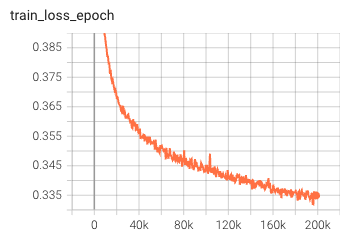
\includegraphics[width=0.4\textwidth]{Figures/protein_training_curve.png}
  \caption{Training loss vs. training epochs. We find that our training is stable in practice.}
  \vspace{-10pt}
  \label{fig:protein-loss-curve}
\end{figure}


\subsection{The Implementation of $\clG$-Equivariant Vector Field}
In \thmref{so3-diffusion}, we require that the vector field is $\SO(3)$-equivariant. In practice, this can be implemented by using a $\SO(3)$-equivariant network architecture or applying data augmentation. In this subsection, we justify that both of these choices are valid, such that the diffusion model can generate a $\SO(3)$-invariant distribution.

\paragraph{Diffusion model with data augmentation.} The optimal solution of the Euclidean diffusion model is given by $\bfD_{\theta}^*(\bfxx_t)=\bbE[\bfxx_1|\bfxx_t]$~\citep{song2021score,karras2022elucidating}. When the data distribution is augmented by random rotation, the data distribution becomes SO(3)-invariant. Thus, the optimal diffusion model can recover the $\SO(3)$-invariant data distribution. When the transition density $p(\bfxx_t|\bfxx_1)$ is $\SO(3)$-equivariant, \ie $p(\bfxx_t|\bfxx_1)=p(g\cdot\bfxx_t|g\cdot\bfxx_1),\forall g\in\SO(3)$, the optimal network is $\SO(3)$-equivariant. To see this, let $g\in\SO(3)$ be an arbitrary rotation matrix. Since
    $\bfD_{\theta}^*(g\cdot\bfxx_t)=\bbE[\bfxx_1|g\cdot\bfxx_t]$,
by the Bayes formula,
\begin{align}
    \bbE[\bfxx_1|g\cdot\bfxx_t]&=\frac{\bbE_{p_\target(\bfxx_1)}[\bfxx_1p(g\cdot\bfxx_t|\bfxx_1)]}{\bbE_{p_\target(\bfxx_1)}[p(g\cdot\bfxx_t|\bfxx_1)]}
    =\frac{\bbE_{p_\target(\bfxx_1)}[\bfxx_1p(\bfxx_t|g^{-1}\cdot\bfxx_1)]}{\bbE_{p_\target(\bfxx_1)}[p(\bfxx_t|g^{-1}\bfxx_1)]}\\
    &=\frac{g\cdot\bbE_{p_\target(g^{-1}\bfxx_1)}[g^{-1}\bfxx_1p(\bfxx_t|g^{-1}\cdot\bfxx_1)]}{\bbE_{p_\target(g^{-1}\bfxx_1)}[p(\bfxx_t|g^{-1}\bfxx_1)]}
    = g\cdot\bbE[\bfxx_1|\bfxx_t],
\end{align}
where we use the equivariance property of the transition density to get the second equality and the invariance property of $p_\target$ to get the third equality. Thus, we can conclude that the optimal solution under these conditions is $\SO(3)$-equivariant. \citet{geffner2025proteina} also gives an empirical validation that a well-trained neural network becomes nearly equivariant even if its architecture is not equivariant.


\paragraph{Equivariant architecture.} When the model is required to be $\SO(3)$-equivariant, the optimal solution of the diffusion model is not $\bbE[\bfxx_1|\bfxx_t]$. To figure out the optimal solution, we consider the training loss at time $t$. The loss function at $t$ is given by
\begin{align}
    \clL_t(\theta)&=\bbE\Vert\bfD_{\theta}(\bfxx_t,t)-\bfxx_1\Vert^2 \\
    &=\int\dd^{3N}\bfxx_1\int\dd^{3N}\bfxx_t \quad p(\bfxx_1,\bfxx_t)\left(\Vert\bfD_{\theta}(\bfxx_t,t)\Vert^2+ \Vert\bfxx_{1}\Vert^2-2\langle\bfD_{\theta}(\bfxx_t,t),\bfxx_1\rangle\right).
\end{align}
The optimal solution satisfies
\begin{align}
    \bfD_{\theta}^*(\bfxx_t,t)=\argmin_{\bfD_{\theta}  \text{ is $\SO(3)$-equivariant}} \clL_t(\theta).
\end{align}
The training loss can be simplified using the equivariant constraint:
\begin{align}
    \clL_t(\theta)&=\int\dd^{3N}\bfxx_1\int\dd^{3N}\bfxx_t ~p(\bfxx_1,\bfxx_t)\left(\Vert\bfD_{\theta}(\bfxx_t)\Vert^2+ \Vert\bfxx_{1}\Vert^2-2\langle\bfD_{\theta}(\bfxx_t),\bfxx_1\rangle\right)\\
    &=\int_{\clM/\SO(3)} \dd \bfrr_t\int_{\SO(3)} \dd g \int\dd^{3N}\bfxx_1 ~p(\bfxx_1,g\cdot \bfrr_t)\left(\Vert\bfD_{\theta}(g\cdot \bfrr_t)\Vert^2+ \Vert\bfxx_{1}\Vert^2-2\langle\bfD_{\theta}(g\cdot \bfrr_t),\bfxx_1\rangle\right),
\end{align}
where $\clM$ is defined in \appxref{r3N-se3-construction}, and $\bfrr_t \in \bbR^{3N}$ is a representation of a quotient-space element in the original Euclidean space.
Since $\bfD_\theta$ is $\SO(3)$-equivariant, $\bfD_{\theta}(g\cdot \bfrr_t) = g \cdot \bfD_{\theta}(\bfrr_t)$, then we have
\begin{align}
    \clL_t(\theta)&=\int_{\clM/\SO(3)} \dd \bfrr_t\int_{\SO(3)} \dd g \int\dd^{3N}\bfxx_1 ~p(\bfxx_1,g\cdot \bfrr_t)\left(\Vert\bfD_{\theta}(\bfrr_t)\Vert^2+ \Vert\bfxx_{1}\Vert^2-2\langle g\cdot\bfD_{1\theta}( \bfrr_t),\bfxx_1\rangle\right).
\end{align}
Define $p(\bfrr_t)=\int_{\SO(3)} \dd g \int\dd^{3N}\bfxx_1 ~p(\bfxx_1,g\cdot \bfrr_t)$, and $p(\bfxx_1, g\mid \bfrr_t)=\frac{p(\bfxx_1,g\cdot\bfrr_t)}{p(\bfrr_t)}$. Then we have
\begin{align}
    \clL_t(\theta)&=\int_{\clM/\SO(3)} \dd \bfrr_t \left[p(\bfrr_t)\Vert\bfD_{\theta}(\bfrr_t)\Vert^2 -2\langle \bfD_{\theta}(\bfrr_t),\int_{\SO(3)} \dd g \int\dd^{3N}\bfxx_1 ~ p(\bfxx_1,g\cdot \bfrr_t) g^{-1}\cdot\bfxx_1\rangle\right] \\
    &+\int_{\clM/\SO(3)} \dd \bfrr_t\int_{\SO(3)} \dd g \int\dd^{3N}\bfxx_1 ~ p(\bfxx_1,g\bfrr_t)\Vert\bfxx_{1}\Vert^2.
\end{align}
So we can conclude that
\begin{align}
    \bfD_{\theta}^*(\bfrr_t,t)&=\int_{\SO(3)} \dd g \int\dd^{3N}\bfxx_1 ~~p(\bfxx_1,g\mid \bfrr_t)~ g^{-1}\cdot \bfxx_1, \\
    \bfD_{\theta}^*(g'\cdot \bfrr_t)&=\int_{\SO(3)} \dd g\int\dd^{3N}\bfxx_1 ~~p(\bfxx_1,g\mid \bfrr_t)~ g'\cdot g^{-1}\cdot \bfxx_1, \forall g \in \SO(3).
\end{align}
Notice that
\begin{align}
    \bfD_{\theta}^*(\bfrr_t)&=\int_{\SO(3)} \dd g \int\dd^{3N}\bfxx_1 ~~p(\bfxx_1,g\mid \bfrr_t)~ g^{-1}\cdot \bfxx_1\\
    &=\frac{\int_{\SO(3)} \dd g \int\dd^{3N}\bfxx_1 ~~p(g\cdot\bfxx_1)p(g\cdot \bfrr_t\mid g\cdot\bfxx_1)\bfxx_1}{\int_{\SO(3)} \dd g \int\dd^{3N}\bfxx_1 ~~p(g\cdot\bfxx_1)p(g\cdot \bfrr_t\mid g\cdot\bfxx_1)}\\
    &=\frac{\int_{\SO(3)} \dd g \int\dd^{3N}\bfxx_1 ~~p(g\cdot\bfxx_1)p(\bfrr_t\mid \bfxx_1)\bfxx_1}{\int_{\SO(3)} \dd g \int\dd^{3N}\bfxx_1 ~~p(g\cdot\bfxx_1)p(\bfrr_t\mid \bfxx_1)},
\end{align}
which is equivalent to the case $p_{\text{data}}=\int_{\SO(3)}\dd g ~~p(g\cdot\bfxx_1)$, \ie using the augmentation by random $\SO(3)$ rotation.

\subsection{Training and Sampling Acceleration}
\begin{figure*}[t]
  \vspace{-2pt}
  \begin{subfigure}[b]{0.50\textwidth}
    \centering
    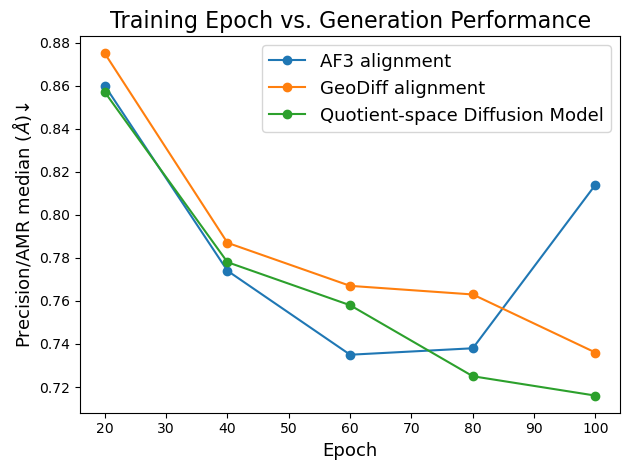
\includegraphics[width=\textwidth]{Figures/training_acc.png}
    \captionsetup{skip=2pt}
    %\caption{}
  \end{subfigure}
  \hspace{-2pt}
  \begin{subfigure}[b]{0.47\textwidth}
    \centering
    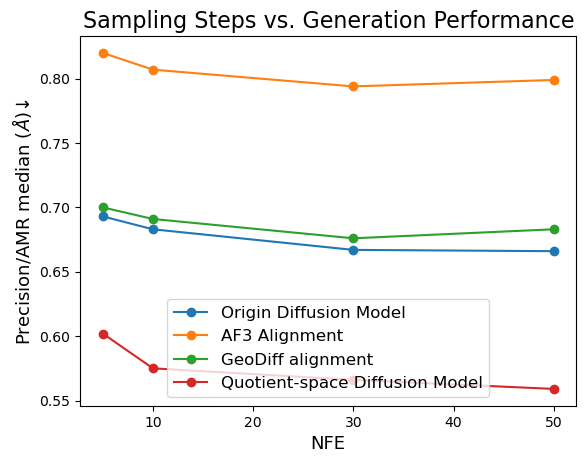
\includegraphics[width=\textwidth]{Figures/sampling_acc.png}
    \captionsetup{skip=2pt}
    %\caption{}
  \end{subfigure}
  \hspace{-2pt}
  \vspace{-4pt}
  \caption{Training and sampling convergence speed comparison on GEOM-DRUGS.
  \textbf{(Left)} The relationship between training epochs and generation performance measured by the precision AMR median metric. 
  \textbf{(Right)} The relationship between the number of function evaluations (NFE) for sampling and generation performance measured by the precision AMR median metric. 
  }
  \label{fig:acc}
\end{figure*}
In this subsection, we study the training and sampling convergence speed of different methods. For the training convergence speed comparison, we plot the generation performance measured by the precision AMR median metric with respect to the training epochs for previous heuristic alignment methods and our quotient-space diffusion model in \figref{acc}(Left). We only focus on the first 100 epochs for all the methods. These models are trained with the same architecture ET-Flow ($\SO(3)$) and training configurations on the GEOM-DRUGS dataset. The results indicate that our method achieves a similar convergence speed to the AF3 heuristic method, because both methods reduce the learning difficulty of the model, as shown in \tabref{comparison}. This theoretical benefit leads to faster convergence than the GeoDiff alignment method. We also notice that the AF3 alignment method starts to get worse generation performance after 80 training epochs. This happens due to the incompatibility between the training loss and the generation performance metric, as the AF3 method is originally designed for the protein structure prediction task, which is not evaluated by distributional metrics.

For the sampling convergence speed comparison, we plot the generation performance measured by the precision AMR median metric with respect to the number of function evaluations (NFE) for the sampling process in \figref{acc}(Right). For all these methods trained on the GEOM-DRUGS dataset, we use the Flow Matching ODE sampler \citep{lipman2023flow} with Euler discretization. From the results, we can observe that models trained with different strategies exhibit similar convergence trends (performance gradually degrades as NFE decreases), our quotient-space diffusion framework consistently outperforms all baselines across every NFE setting. 

\subsection{Quotient Space beyond $\bbR^{3N}/\SE(3)$}
Our framework can generalize to 
quotient spaces generated by symmetry groups beyond the special Euclidean group $\mathrm{SE}(3)$. Possible examples include the $\mathrm{U}(1)$ symmetry in quantum wavefunctions, the $\mathrm{SU}(2)$ symmetry in particle physics, 
and the $\mathrm{SO}(3)$ symmetry in higher ($>3$) representation spaces for tasks including the mean-field electron Hamiltonian matrix prediction.
In this work, we focus on the $\mathrm{SE}(3)$ case for its significant relevance to scientific research \citep{abramson2024accurate}. Applications of our framework on the mentioned more diverse systems above are left as future work.

\section{Experiments}\label{appx:experiments}
\subsection{Molecular Structure Generation}\label{appx:geom}
This appendix summarizes our experimental setup, which strictly follows that of ET-Flow~\citep{hassan2024flow}.
We detail the datasets, model architecture, training, sampling, and evaluation. 
For a more comprehensive discussion of each component, we refer the reader to the appendices of their original paper.

\textbf{Dataset.}  First, we evaluate our framework on the molecule structure generation task. In this scenario, our goal is to generate the 3D coordinates of a molecule given the graph structure of the molecule. We conduct the experiments on the GEOM datasets~\citep{axelrod2022geom}, which provide structure ensembles generated by metadynamics in CREST~\citep{pracht2024crest}, and we focus on the GEOM-QM9 and GEOM-DRUGS datasets. Following the data processing and splits from \citep{hassan2024flow}, we use the random splits with train/validation/test of 243473/30433/1000 for GEOM-DRUGS and 106586/13323/1000 for GEOM-QM9. In addition, data with disconnected molecule graphs are removed for GEOM-DRUGS \citep{hassan2024flow}. Our reproduction is based on the modified data-processing pipeline following the released configs thus different from the results reported in the original paper.

\paragraph{Settings.} We primarily follow the setting in \citep{hassan2024flow}. We set the Gaussian distribution as the prior distribution on GEOM-QM9 and use the harmonic prior for GEOM-DRUGS \citep{volk2023alphaflow}. Following \citep{jing2022torsional,xu2022geodiff}, we report the RMSD-based metrics, \eg Coverage and Average Minimum RMSD (AMR) between generated and ground truth structure ensembles. We parameterize $\bfvv_{\theta}$ by using equivariant graph transformer architectures from ET-Flow~\citep{hassan2024flow}, including the O(3) and SO(3) equivariant variants, which also serves as a verification that our framework is compatible with different backbone models. For training,  we use AdamW as the optimizer, and set the hyper-parameter $\epsilon$ to 1e-8 and $(\beta_1,\beta_2)$ to (0.9,0.999). We use the dynamic gradient clipping as~\citep{hassan2024flow,hoogeboom22equivariant}. The peak learning rate is set to 5e-4 for GEOM-DRUGS and 7e-4 for GEOM-QM9. The batch size is set to 48 for GEOM-DRUGS and 128 for GEOM-QM9.  The weight decay is set to 1e-8. The model is trained for 1000 epochs for both datasets. The noise scale $\sigma$ is set to $0.1$. We also use 50 time steps with the Euler solver for sampling. All models are trained on 8 NVIDIA A100 GPUs.

\textbf{Baselines.} Following~\citep{hassan2024flow}, we choose strong baselines trained on GEOM-DRUGS and GEOM-QM9 for a challenging comparison. We report the performance of GeoMol \citep{ganea2021geomol}, GeoDiff \citep{xu2022geodiff}, Torsional Diffusion \citep{jing2022torsional}, and MCF \citep{wang2023swallowing}. 

\subsection{Protein}\label{appx:protein}

This appendix summarizes our experimental setup, which strictly follows that of Prote\'ina~\citep{geffner2025proteina}.
We detail the datasets, model architecture, training, sampling, and evaluation. 
For a more comprehensive discussion of each component, we refer the reader to the appendices of their original paper.

\subsubsection{Dataset}
\label{appx:protein_dataset}
For training, we utilize the Foldseek AFDB clusters ($D_{\text{FS}}$) dataset as curated and described in the Prote\'ina. 
This dataset is a high-quality, non-redundant subset of the AlphaFold Database (AFDB), containing 588,318 cluster-representative protein structures with lengths between 32 and 256 residues. 
The dataset is annotated with hierarchical CATH labels, which are leveraged during training. 
Our data processing and handling strictly follow the pipeline detailed in Appendix M of~\citep{geffner2025proteina}.

\subsubsection{Model Architecture and Training}
\label{appx:protein_model}
Our model architecture is the same as the efficient, non-equivariant transformer proposed by~\citep{geffner2025proteina}. Specifically, we adopt the variant that forgoes the use of computationally expensive triangle update layers.
The model is trained using the conditional flow matching (CFM) objective.
Key aspects of the training protocol from Prote\'ina are preserved, including their novel Beta-Uniform mixture for the time-sampling distribution $p(t)$, the use of self-conditioning, and data augmentation with random rotations.
All model and training hyperparameters, such as embedding dimensions, number of layers, attention heads, and optimizer settings, are kept consistent with hyperparameters saved in their released checkpoint $\mathcal{M}_{\text{FS}}^{\text{small}}$.
The hyperparameters for the $\mathcal{M}_{\text{FS}}^{\text{small}}$ model are detailed in Table~\ref{tab:protein_hyperparameter}, in comparison with the larger models from the original Proteína paper.

\begin{table}[htbp]
\centering
\caption{Hyperparameters for Prote\'ina model.}
\label{tab:protein_hyperparameter}
\begin{tabular}{@{}lccc@{}}
\toprule
\textbf{Hyperparameter} & $\mathcal{M}_{\text{FS}}$ & $\mathcal{M}_{\text{FS}}^{\text{no-tri}}$ & $\mathcal{M}_{\text{FS}}^{\text{small}}$ \\
\midrule
\multicolumn{4}{@{}l}{\textbf{Prote\'ina Architecture}} \\
sequence repr dim & 768 & 768 & 512 \\
\# registers & 10 & 10 & 10 \\
sequence cond dim & 512 & 512 & 128 \\
$t$ sinusoidal enc dim & 256 & 256 & 196 \\
idx. sinusoidal enc dim & 128 & 128 & 196 \\
fold emb dim & 256 & 256 & 196 \\
pair repr dim & 512 & 512 & 196 \\
seq separation dim & 128 & 128 & 128 \\
pair distances dim ($x_t$) & 64 & 64 & 64 \\
pair distances dim ($\tilde{x}(x_t)$) & 128 & 128 & 128 \\
pair distances min (\AA) & 1 & 1 & 1 \\
pair distances max (\AA) & 30 & 30 & 30 \\
\# attention heads & 12 & 12 & 12 \\
\# tranformer layers & 15 & 15 & 12 \\
\# triangle layers & 5 & --- & --- \\
\# trainable parameters & 200M & 200M & 60M \\
\midrule
\multicolumn{4}{@{}l}{\textbf{Prote\'ina Training}} \\
\# steps & 200K & 360K & 150K \\
batch size per GPU & 4 & 10 & 5 \\
\# GPUs & 128 & 96 & 16 \\
\# grad. acc. steps & 1 & 1 & 1 \\
\bottomrule
\end{tabular}
\end{table}

\subsubsection{Sampling}
\label{appx:protein_sampling}
To facilitate a direct comparison with the publicly available Prote\'ina checkpoints, we trained our model with an identical hierarchical fold class conditioning mechanism. 
However, to ensure a fair assessment of foundational generative capabilities, all experiments reported in our main text were performed in a strictly unconditional setting.
We applied the same sampling protocol across all models, using 400 sampling steps and enabling self-conditioning, which consistently improved performance. 
No other guidance techniques, such as autoguidance, were utilized. 
We use deterministic ODE sampling to assess distributional fidelity and SDE sampling to explore the designability-diversity trade-off. 
We adapt the SDE formulation and its Euler-Maruyama numerical scheme, detailed in Appendix I of~\citep{geffner2025proteina}, for our quotient space framework, while retaining all other configurations, such as the sampling scheduler and $g(t)$, from the original paper.

\subsubsection{Evaluation}
\label{appx:protein_evaluation}
We evaluate our models rigorously adheres to the metrics established and validated in the Prote\'ina paper.
We assess model performance using the standard suite of metrics in protein design: 
\begin{itemize}
    \item \textbf{Designability.} Quantified by the self-consistency RMSD (scRMSD) protocol, using ProteinMPNN for inverse folding and ESMFold for structure prediction, with a success threshold of scRMSD less than 2\AA.
    \item \textbf{Diversity.} Measured in two ways: by the average pairwise TM-score among designable samples, and by the number of distinct structural clusters identified by Foldseek at a TM-score threshold of 0.5.
    \item \textbf{Novelty.} Assessed by calculating the maximum TM-score of each designable sample against reference structures in the PDB and AFDB databases.
\end{itemize}
We also  adopt the novel probabilistic metrics introduced by~\citep{geffner2025proteina}, to measure how well our model captures the true distribution of protein structures:
\begin{itemize}
    \item \textbf{FPSD.} Measured the distributional similarity between generated and reference structures in the feature space of a pre-trained fold class predictor.
    \item \textbf{fS.} Evaluated both the quality and diversity of samples based on the confidence and entropy of fold class predictions.
    \item \textbf{fJSD.} Quantified the similarity between the categorical fold class distributions of generated and reference sets.
\end{itemize}

It is noteworthy that we have omitted the Diversity and Novelty metrics from our main text to avoid comparisons with potentially inaccurate results in the literature. 
This decision is based on a bug recently identified in the alntmscore output of FoldSeek versions prior to v10 (release 10-941cd33), which renders many previously reported TM-based metrics incorrect (also found in~\citep{daras2025ambient}). 
To provide a controlled and accurate benchmark, we conducted our own analysis using the FoldSeek v10 (release 10-941cd33).
We limited this re-evaluation to the released small Proteína model and our corresponding model trained in the quotient space. The full results of this comparison are summarized in Table~\ref{tab:protein_backbone_full}.

\begin{table}[htbp]
\centering
\footnotesize
\caption{Complete performance comparison of the released Prote\'ina checkpoints against our version in the quotient space. Best results are marked in \textbf{bold}.}
\label{tab:protein_backbone_full}
\vspace{0.3cm}
\resizebox{1.0\textwidth}{!}{%
\begin{tabular}{lccccccccccc}
\toprule
\multirow{2}{*}{Model} & \multirow{2}{*}{Designability (\%)} & \multicolumn{2}{c}{Diversity} & \multicolumn{2}{c}{Novelty vs.} & \multicolumn{2}{c}{FPSD vs.} & fS & \multicolumn{2}{c}{fJSD vs.} \\
\cmidrule(lr){3-4} \cmidrule(lr){5-6} \cmidrule(lr){7-8} \cmidrule(lr){9-9} \cmidrule(lr){10-11}
& & Cluster$\uparrow$ & TM-Sc.$\downarrow$ & PDB$\downarrow$ & AFDB$\downarrow$ & PDB$\downarrow$ & AFDB$\downarrow$ & (C/A/T)$\uparrow$ & PDB$\downarrow$ & AFDB$\downarrow$ \\
\midrule 
\multicolumn{7}{@{}l}{\textbf{SDE Sampling}} \\
$\mathcal{M}_{\text{FS}}^{\text{small}}, \gamma=0.35$& 96.0 & 0.44 (209) & 0.50 & 0.86 & 0.91 & 386.5 & 378.2 & 1.77/4.97/17.78 & 2.17 & 1.73 \\
\rowcolor{gray!25}
$\mathcal{M}_{\text{FS}}^{\text{small}}, \gamma=0.35$ + ours & \textbf{97.6} & 0.40 (197) & 0.48 & 0.86 & 0.91 & 274.7 & 277.1 & 2.24/6.69/20.99 & 1.68 & 1.55 \\
$\mathcal{M}_{\text{FS}}^{\text{small}}, \gamma=0.45$ & 92.2 & 0.55 (253) & 0.49 & 0.84 & 0.90 & 332.9 & 320.4 & 1.83/5.01/20.22 & 1.93 & 1.49 \\
\rowcolor{gray!25}
$\mathcal{M}_{\text{FS}}^{\text{small}}, \gamma=0.45$ + ours & 92.6 & 0.51 (253) & 0.47 & 0.85 & 0.90 & 244.5 & 246.3 & 2.24/6.68/23.47 & 1.43 & 1.28 \\
$\mathcal{M}_{\text{FS}}^{\text{small}}, \gamma=0.50$ & 89.2 & 0.57 (255) & 0.48 & 0.83 & 0.89 & 306.2 & 290.8 & 1.86/4.92/21.15 & 1.81 & 1.36 \\
\rowcolor{gray!25}
$\mathcal{M}_{\text{FS}}^{\text{small}}, \gamma=0.50$ + ours & 90.2 & 0.51 (231) & 0.47 & 0.84 & 0.90 & 228.0 & 228.7 & 2.25/6.59/25.24 & 1.32 & 1.17 \\
\midrule
\multicolumn{7}{@{}l}{\textbf{ODE Sampling}} \\
$\mathcal{M}_{\text{FS}}^{\text{small}}$ & 13.8 & 0.90 (62) & 0.43 & 0.80 & 0.87 & 83.18 & 21.93 & 2.45/5.63/31.76 & 0.58 & 0.12 \\
\rowcolor{gray!25}
$\mathcal{M}_{\text{FS}}^{\text{small}}$ + ours & 15.6 & 0.87 (68) & 0.43 & 0.80 & 0.86 & \textbf{69.94} & \textbf{17.56} & \textbf{2.57/6.40/32.14} & \textbf{0.41} & 0.11 \\
\bottomrule
\end{tabular}%
}
\end{table}
